%% Encoding: UTF-8

% 字号选项: c5size 五号(默认) cs4size 小四
% 双面打印(注意字号设置)
% \setCJKmainfont[SmallCapsFont=*]{Adobe Song Std}
% 单面打印(注意字号设置)
% \documentclass[cs4size, a4paer, oneside, openany]{sjtuthesis} 
\documentclass[cs4size, a4paper, twoside]{sjtuthesis} 

% \usepackage[sectionbib]{chapterbib}%每章都用参考文献

\usepackage[lined,boxed,commentsnumbered,ruled,linesnumbered]{algorithm2e}
\usepackage[normalem]{ulem}
\usepackage{enumitem}
\usepackage{multicol,pdflscape}
\usepackage{subfigure}
\addtolength{\subfigcapskip}{-24pt}
% \usepackage[dvipsnames]{xcolor}
\definecolor{mygreen}{rgb}{0,0.6,0}
\definecolor{mygray}{rgb}{0.5,0.5,0.5}
\definecolor{mymauve}{rgb}{0.58,0,0.82}
\lstset{ %
  backgroundcolor=\color{white},   % choose the background color; you must add \usepackage{color} or \usepackage{xcolor}
  basicstyle=\ttfamily\footnotesize,        % the size of the fonts that are used for the code
  breakatwhitespace=false,         % sets if automatic breaks should only happen at whitespace
  breaklines=true,                 % sets automatic line breaking
  captionpos=b,                    % sets the caption-position to bottom
  commentstyle=\color{mygray}\itshape,    % comment style
  deletekeywords={...},            % if you want to delete keywords from the given language
  escapeinside={\%*}{*)},          % if you want to add LaTeX within your code
  extendedchars=true,              % lets you use non-ASCII characters; for 8-bits encodings only, does not work with UTF-8
%  frame=single,                    % adds a frame around the code
  keepspaces=true,                 % keeps spaces in text, useful for keeping indentation of code (possibly needs columns=flexible)
  keywordstyle=\color{blue},       % keyword style
  identifierstyle=\texttt,
  language=C,                      % the language of the code
  morekeywords={*,...},            % if you want to add more keywords to the set
  numbers=left,                    % where to put the line-numbers; possible values are (none, left, right)
  numbersep=5pt,                   % how far the line-numbers are from the code
  numberstyle=\tiny\color{mygray}, % the style that is used for the line-numbers
  rulecolor=\color{black},         % if not set, the frame-color may be changed on line-breaks within not-black text (e.g. comments (green here))
  showspaces=false,                % show spaces everywhere adding particular underscores; it overrides 'showstringspaces'
  showstringspaces=false,          % underline spaces within strings only
  showtabs=false,                  % show tabs within strings adding particular underscores
  stepnumber=1,                    % the step between two line-numbers. If it's 1, each line will be numbered
  stringstyle=\color{mymauve},     % string literal style
  tabsize=2,                       % sets default tabsize to 2 spaces
  title=\lstname                   % show the filename of files included with \lstinputlisting; also try caption instead of title
}

\newboolean{DOIT}
\setboolean{DOIT}{false}%编译某些只想自己看的内容,编译true,否则false

%% 行距缩放因子(x倍字号)
\renewcommand{\baselinestretch}{1.3}

% 设置图形文件的搜索路径
\graphicspath{{figure/}{figures/}{logo/}{logos/}{graph/}{graphs}}

%%==============================================================================
%% 在sjtuthesis.cls中定义的有用命令
%%==============================================================================
% \cndash 中文破折号
% 数学常量
% \me 对数常数e
% \mi 虚数单位i
% \mj 虚数单位j
% \dif 直立的微分算符d为直立体。
% 可伸长的数学箭头、等号
% \myRightarrow{}{}
% \myLeftarrow{}{}
% \myBioarrow{}{}
% \myLongEqual{}{}
% 参考文献
% \upcite{} 上标引用
%%==============================================================================

\newcommand{\todo}[1]{{\footnotesize \textcolor{red}{$\ll$\textsf{TODO #1}$\gg$}}}
\newcommand{\dryrun}{\textsf{SERAPH}}
\newcommand{\rbscope}{\texttt{rbscope}}

\newcommand{\bug}{\ensuremath{\mathcal{B}}}
\newcommand{\patch}{\ensuremath{\mathcal{P}}}
\newcommand{\prog}{\ensuremath{\mathcal{S}}}
\newcommand{\bs}{\ensuremath{_{bug}}}
\newcommand{\ass}{\ensuremath{_{assert}}}
\newcommand{\entry}{\ensuremath{_{entry}}}
\newcommand{\ps}{\ensuremath{_{root}}}
\newcommand{\scope}{\ensuremath{_{scope}}}
\newcommand{\pin}{\ensuremath{V_{inputs}}}

\begin{document}

% 中文封面内容
\title{基于选择性符号执行的补丁验证}
\author{陈\quad{}泓\quad{}旭}
\advisor{赵建军教授}
\degree{硕士}
\defenddate{2014年1月7日}
\school{上海交通大学}
\institute{软件学院}
\studentnumber{1110379002}
\major{计算机科学与技术}

% 英文封面内容
\englishtitle{Selective Symbolic Execution Based Patch Validation}
\englishauthor{\textsc{Hongxu Chen}}
\englishadvisor{Prof. \textsc{Jianjun Zhao}}
\englishschool{Shanghai Jiao Tong University}
\englishinstitute{\textsc{School of Software} \\
  \textsc{Shanghai Jiao Tong University} \\
  \textsc{Shanghai, P.R.China}}

\englishdegree{Master}
\englishmajor{Computer Science and Technology}
\englishdate{Jan. 7th, 2014}

%% 生成封面
\maketitle

\makeenglishtitle

% 论文原创性声明和使用授权
\makeDeclareOriginal

\makeDeclareAuthorization

%% 前言
\frontmatter

% 摘要
\begin{abstract}
Something pithy.
\end{abstract}


% 目录
\tableofcontents

% 表格索引
\listoftables

% 插图索引
\listoffigures

\addcontentsline{toc}{chapter}{\listtablename}  %将图索引加入全文目录
\addcontentsline{toc}{chapter}{\listfigurename} %将表格索引加入全文目录

\def\chapterautorefname~#1\null{第{#1}章\null}
\def\sectionautorefname~#1\null{#1~小节\null}
\def\subsectionautorefname~#1\null{#1~小节\null}
\def\subsubsectionautorefname~#1\null{#1~小节\null}
\renewcommand\figureautorefname{图}
\renewcommand\tableautorefname{表}
\renewcommand\appendixautorefname{附录}%
\renewcommand{\algorithmcfname}{算法}

% 主要符号、缩略词对照表
\chapter{主要符号对照表}
\label{chap:symb}

\begin{tabular}{ll}

  \hspace{2em}\bug           &     \hspace{5em}原有的含错误的程序 \\
  \hspace{2em}\patch         &     \hspace{5em}修改过的补丁程序 \\
  \hspace{2em}\prog          &     \hspace{5em}一般意义下的程序 \\
  \hspace{2em}\prog\bs       &     \hspace{5em}程序\prog 中触发错误的位置 \\
  \hspace{2em}\prog\ass      &     \hspace{5em}程序\prog 中所关注的assert宏位置 \\
  \hspace{2em}\prog\ps       &     \hspace{5em}程序\prog 中导致错误发生原因的位置\\
  \hspace{2em}\prog\entry    &     \hspace{5em}所指定的程序\prog 的入口函数\\
  \hspace{2em}\prog\scope    &     \hspace{5em}由\prog\entry 、\prog\ps 、\prog\bs 得到的\rbscope \\
  \hspace{2em}\pin          &     \hspace{5em}给某个程序的一个输入值向量


\end{tabular}


%%==============================================================================
%% 正文
%%==============================================================================
\mainmatter

%% 各章正文内容
\chapter{绪论}
\label{chap:intro}

\section{研究背景}
\label{sec:background}

\subsection{课题的研究意义}
\label{sec:meaning}

补丁验证是一个正日益受到学术界和工业界关注的问题~\upcite{apsys12, fixation, dora},它能有效地防止包含错误的程序补丁被不适当地添加进新版本程序代码中。

软件开发过程中,经常需要对含有错误(臭虫,bug)的程序提交补丁(patch)。然而错误的补丁有可能是不完全的,即:该程序补丁仅修复了部分程序输入导致的程序错误,但对于另外一些可能的输入仍然会引发错误。另一方面,这些补丁可能是一些回归补丁(regression patch),它引发了在原有程序中不存在的新的错误。更有甚者,这些补丁可能兼有这两种错误。错误补丁的存在使得程序不再健壮,甚至会增加后续过程中产生正确的补丁的难度。

为此,业界需要采取有效的方法来验证经过修改的程序的正确性。在理论上可以通过形式化证明、静态分析和软件测试等方法来提高补丁的可靠性。形式化证明的方法可以完全地验证程序的正确性,然而由于软件所使用程序语言本身的复杂性,且基于理论推导的验证过程时间开销很大,该方法通常不能用于现实中的程序。语法上的分析可以检测语法错误或潜在的可能的语义错误,一般的编译器前端可以检测这类较为低级的错误;通过数据流、控制流、指向分析等静态分析的手段可以检测出程序中如变量越界等典型错误,然而这些方法检测的错误类型仍然极其有限。因此通常仅采用轻量级的静态分析作为辅助检测程序错误的手段。

现实中往往通过人工编写大量的测试用例进行测试以提高软件的质量。手动编写测试的本身存在一些不可避免的问题。首先,测试用例往往不能达到较高的语句覆盖率;现实中测试人员对待测程序理解不够深入,难以生成绝大多数可行的程序输入,分支覆盖率和路径覆盖率很低。对补丁程序的不完整测试会带来严重的后果,一个不正确的补丁可能会隐藏原先的错误所在,使其更为隐蔽,大大增加得到最终正确补丁的难度。近期的一项研究结果表明,大约$14.8\%$-$25\%$的补丁是不正确的~\upcite{BuggyFix}。 事实上,有$38\%$-$50\%$的Bugzilla数据库\footnote{Bugzilla首页: http://www.bugzilla.org/}中的bug被重新打开(reopen)~\upcite{fixation}。对完整的待验证补丁程序进行高覆盖率的测试需要很大的时间开销。这一过程通常包含多种测试手段,包括单元测试、回归测试,有时还需要压力测试;这极有可能会要求更大的测试用例集合。然而如果对程序补丁的验证不够及时,一般会直接导致程序员生产效率的下降。这是因为该过程是软件演化过程中的一个关键步骤,它需要不断迭代进行,这是一个交互的过程。一项研究~\upcite{maintenance}表明,程序员花费了$50\%$-$80\%$的时间用于检测、定位故障并修正错误。因此,工业界迫切需要有一种既能够提高补丁验证质量又可以加速自动验证的新技术。

近些年来符号执行(symbolic execution)在生成高覆盖率的测试用例集和发现复杂软件中潜在错误上有了新的突破,正日益受到研究人员和工业界的关注。其基本思想是用符号值而不是具体值作为程序的输入进行执行,根据执行路径上不同的路径条件(path condition),藉由约束求解器(constraint solver)来验证条件是否可行;当得知该条件可以满足时,将符合该条件约束的所有可行的值作为原有程序的输入进行具体的程序执行。由于该过程类似于以可行的程序输入真实动态执行程序本身,故从理论上来说符号执行可以检测出程序中可能发生的任何错误,对静态分析方法无法检测的错误检测尤为有效。由于当前技术水平限制,现有符号执行工具都不是完全意义上的符号执行,然而比起基于手工的测试仍会有更高的覆盖率~\upcite{KLEE}。

由于svn,git等软件配置管理(Software Configuration Management)工具的普及,人们可以方便地追踪程序变化历史。
在对国内外知名代码仓库中的bug提交结果分析之后,我们发现补丁程序和原有含有错误的程序的改动相对不大,程序补丁往往仅修复单个错误,其影响通常限于程序的局部~\upcite{APSYS11},且很少涉及程序的核心语义~\upcite{DeltaExecution}。这使得没有必要对整个程序使用符号执行的工具验证。同时,由于符号执行的路径爆炸(path explosion)及约束求解器的限制,对现实中的程序完整地进行符号执行也是不可行的。

基于上述观察,本课题提出有选择性的符号执行方法以验证所给补丁正确性,力求减少时间上的开销。首先依据程序的改动部分(patch site)和原有程序错误发生节点(bug site)作为配置信息,基于指向分析方法,利用调用图信息、程序可达性信息及影响性结果,削减不相关程序,得到仅和补丁及原有错误相关的程序片段,添加符号执行的语义和驱动程序,通过对这一程序子集合进行符号执行以检测原有程序中可能存在的错误。

\subsection{国内外研究现状}
\label{sec:current}
符号执行(symbolic execution)的基本思想最早于上世纪80年代由Robert S.Boyer等人提出~\upcite{SELECT}, 后经James C. King等~\upcite{EFFIGY}加以精化并应用于软件测试领域。然而由于经典的符号执行没有高效的算法实现、当时计算机计算能力有限等因素制约,符号执行不能应用于现实程序中。

针对符号执行的路径爆炸、求解器约束等问题,自2000年以来,学者们针对测试用例生成这一场景,从不同角度提出了提高符号执行覆盖率的方法,增强了检测程序bug的能力。

首先是在符号执行模型上的改进。现代的符号执行系统一般有如下两种类型。
\begin{itemize}
\item “将具体输入和符号执行结合”的方法,由P. Godefroid等人于2005年提出,最早应用于执行工具DART~\upcite{DART}中。和经典符号执行的方法不同,DART采用随机生成的具体值(concrete value)作为程序输入,在每一个可能的程序分叉处,取反给定的输入值的分支约束条件,通过约束求解器计算与当前输入值不同的路径,以实现对路径的遍历。这种将具体值(CONCrete)和符号值(symbOLIC)结合执行的生成测试用例的方法又被称作CONCOLIC Testing。这样的执行会使得部分可行的分支条件被忽略而遗漏很多可行的执行路径,但是却能部分解决原本约束求解器无法求解的非线性约束,提高了符号执行的速度。由此诞生的另外一些工具如DiSE~\upcite{DiSE}、CUTE~\upcite{CUTE}、jCUTE~\upcite{CUTE}、SAGE~\upcite{SAGE}也基于这一思想。
  \item “由执行生成测试”(Execution-Generated Testing,EGT)的方法,其典型实现为EXE~\upcite{EXE}和KLEE~\upcite{KLEE}。EGT工具把符号值作为程序的输入,在每一处可能产生错误的危险操作上计算可能的条件,由约束求解器得到符号的约束条件并给出可行的具体值,从而生成不同的具体程序状态(states)。EGT在每一含有确定具体值的语句处对程序进行解释执行;当符号执行工具察觉到约束求解器无法求解约束条件时(如遇到外部函数调用或浮点型比较),则使用具体值带入执行。基于这一方法的应用有DDT~\upcite{kuznetsov2010testing},ESD~\upcite{zamfir2010execution},RevNIC~\upcite{chipounov2010reverse}等。
\end{itemize}

另一个研究方向是对于需要符号执行的程序的片段的选择性执行上的优化。对大型程序符号执行的代价较大,但实际情形中往往仅需对小部份程序进行验证。
\begin{itemize}
\item Vitaly Chipounov等人给出了$S^2E$这样一个分析程序的平台~\upcite{S2E},使得可以通过用户选用不同粒度的符号执行策略对程序进行验证;例如$S^2E$可以选择是否对指定库函数进行符号执行、如何执行外部函数等,这也使得对不能得到源代码的二进制程序进行符号执行成为可能。
\item Woodpecker~\upcite{WOODPECKER}是另一类有选择的符号执行方法,它只关注程序中的一些特定规则(如打开的文件在程序结束前必须关闭等),使用符号执行对这些规则进行验证;由于特定规则会有一些特定模式,可以避免在所有路径上符号执行。
\end{itemize}

\section{研究内容}
\label{sec:brief}

\subsection{课题的研究目标}
\label{sec:goal}

静态分析和符号执行都有其自身的优势及缺陷。静态分析可以在不执行程序的前提下检测程序中可能的错误,这避免了程序执行带来的破坏;它是完全的(complete)但并不充分(sound):只有当没有一条可行的路径会运行至程序的错误节点~\upcite{rule}或触发该错误的最弱前置条件(weakest precondition)不可满足~\upcite{fixation}才认为该路径是正确的;否则它仅仅保守地警告可能的错误补丁而不提供精确的运行时信息。因此这会产生大量的错误肯定(false positive),并且由于不能得到触发错误的具体程序输入,很多情况下会增大而非减少程序员的负担。另一方面,因为符号执行真实执行符号化的程序输入,这使得其结果是充分的。由于其具体值的求解是由约束求解器(constraint solver)完成的,这往往会比人工编写的测试用例具有更高的覆盖率,从而比手工测试更为完全~\upcite{ContinuousTest, dora};和静态分析相反,符号执行引擎总可以得到引发错误的具体输入值。

纯静态分析和符号执行都面临着扩展性问题。对于大中型规模的程序而言,它们通常都需要相当长的时间才可以完成。为了取得精确的结果,静态分析需要得到流敏感(flow sensitive)、上下文敏感(context sensitive)甚至路径敏感(path sensitive)的分析结果,这使得静态方法对大型复杂程序束手无策。对大规模的程序进行符号执行的代价也是巨大的,状态爆炸(path explosion)使得符号执行工具难以获得高的语句覆盖和分支覆盖,约束求解器求解约束条件的限制使得在理论上无法对部分程序进行符号执行。

我们针对软件演化这一场景,希望通过选择性符号执行的方法仅对补丁程序中的相关部分进行符号执行,结合静态分析和动态符号执行各自的优势,正确且高效地对补丁进行验证。
我们的研究目标如下:
\begin{enumerate}
\item 在大部分情况下,当补丁程序存在错误时,有选择的符号执行须比一般的符号执行工具花费更少的时间检测出程序中的错误。
\item 有选择的符号执行在检测出错误时需要得到触发该错误的测试用例,将之带入原有的完整程序中时,需要正确触发程序中的错误。
\item 当补丁程序存在错误时,需进一步分析该错误是回归错误或是由于补丁只修复了部分错误造成的。
\item 当程序补丁是正确的情况下,选择性符号执行不应该得到该补丁程序存在错误这一结论。
\end{enumerate}

然而由于符号执行自身的局限性,且选择性符号执行因为不是验证程序本身而是程序的相关子集,因此上述目标往往不能完全实现。

\subsection{本文的工作}
\label{sec:contr}

我们建立了\dryrun\footnote{\dryrun 是“守护者”的意思, 也是Symbolic Execution Represents A PHase的缩写。}补丁验证系统,它结合了静态分析和基于动态符号执行的自动化测试的优点,大大提高了程序的可扩展性。\dryrun 核心思想较为简单:
\begin{enumerate}
\item 将问题定位到所做补丁处及错误发生处的所有可能的程序执行路径,并进一步通过静态分析的方法去除和补丁修改无关的部分和不影响错误发生的程序片段,最终得到一个局部的程序片段。该片段被称为 \rbscope ,其含义为出错程序的根本原因(Root cause)和程序出错点(Bug site)的区域(SCOPE)。
\item 给\rbscope 添加对应的入口函数信息,并添加符号执行的语义,得到符号执行引擎可以执行的编译单元。使用符号执行引擎对该程序片段解释执行,通过符号执行的结果判断所做补丁的正确性。同时,为分析补丁程序和原有程序的关系(即交叉验证),将前述静态分析应用于未添加补丁的程序,并通过类似方法将未修改程序添加入符号分析工具执行的编译单元中。这样可以根据两个版本程序间路径\cndash 路径关系的比较结果,判断bug是否已被修复、仅部分被修复或补丁引发了新的错误。
\end{enumerate}

因为没有考虑到\rbscope 之外程序的准确前置条件,这样的方法仍然是不充分的;然而,由于完整性和速度方面的提升,使得这一权衡是值得的。\dryrun 通过对十多个GNU Coreutils(详见\autoref{chap:eval}\nameref{chap:eval})中的错误补丁进行检测,找到了所有的补丁错误,和KLEE对完整程序执行相比,最高可达到1000倍左右的性能提高。

% --------------------------------------------

本课题是建立在静态分析框架LLVM和符号执行器KLEE的基础上的,我们希望给定bug程序和其补丁程序,经过一系列地中间代码转化,生成一份LLVM指令代码文件作为KLEE的输入,在符号执行结束后分析补丁程序的正确性以及是否引入新的错误等;如果该补丁并不正确,还需要得到引发程序错误的输入用例。

为了实现该课题的研究目标,研究主要集中在以下五方面的内容:
\begin{enumerate}[label={(\arabic*)}]
\item 理解LLVM中间表达形式(LLVM IR)的组成,掌握生成、分析、转化中间代码的基本方法。
\item 在LLVM中间代码上根据Andersen指向算法,给出编译单元内调用图和修改集合信息。
\item 基于对程序补丁处及程序错误发生处的过程间可达性分析削减程序中的不可达部分。
\item 以程序出错位置作为后向切片准则, 实现所给程序范围内的后向切片, 保留从程序片段入口处可能影响程序出错处的指令集合。
\item 通过程序转化,在中间代码层次给程序添加符号执行引擎可理解的语义及程序入口,生成符号执行的驱动程序。
\end{enumerate}

本论文的主要贡献如下:
\begin{itemize}
\item 提出了一种新的补丁验证的方法,使得可以通过有选择的符号执行对补丁进行有效并高效地验证。
\item 计算所有可能的从补丁处至错误发生处的极小相关程序范围。
\item 给出了如何由现有程序的\rbscope 生成可供验证驱动程序进行交叉验证的算法,使得可以通过符号执行结果对“补丁程序是否完整或引入新的错误”这一问题给出正确解释。
\item 实现了该思想的工具原型\dryrun ,使得可以对Coreutils等实际复杂程序中的补丁进行验证。
\end{itemize}

\section{本文的内容组织}
\label{sec:struct}
本文共包括六章,各章的内容组织如下:
\begin{itemize}
\item 第一章是文章的绪论部分。主要说明本课题的研究意义,分析相关领域的国内外研究现状,然后介绍课题的研究目标以及所做的工作;最后说明了本文的组织结构。
\item 第二章从宏观上介绍了有选择性符号执行验证技术,这是\dryrun 工具的理论基础。本章详细阐述了静态分析技术结合符号执行的理论基础及现有的可用基础框架,首先解释了符号执行工具的基本概念及具体应用,之后介绍了建立在LLVM中间表达形式上的符号执行引擎KLEE的原理,最后通过一个具体的例子说明了有选择符号执行用于程序验证的场景。
\item 第三章是\dryrun 的前半部分实现,介绍了\rbscope 的生成过程,主要介绍将程序中的不相关部分通过静态分析进行删减的方法。详细说明了\rbscope 生成流程图的方法,接着着重介绍了关注点配置、指向分析、调用图的生成等用于程序转化的准备工作,最终分别阐述了基于未调用函数的削减、基于程序可达性的削减及基于程序影响性分析的削减方法。
\item 第四章是补丁验证,是\dryrun 的后半部分实现。解释了如何根据\rbscope 使用代码转化技术合成为符号执行工具可理解的程序并对之验证,同时给出了交叉验证的算法;最终针对一类难以进行符号执行的程序提出了使用用户提供初始化的方法来辅助验证的方案。
\item 第五章是实验与评估。首先给出了\dryrun 用于补丁验证的一般实验流程。之后介绍了具体的实验方案:从类Unix系统下常用的Coreutils的程序集中无差别地选取数十个程序并手工添加补丁,评估了\dryrun 验证补丁的正确性和高效性,同时分析了\dryrun 带来的错误肯定(false positive)及交叉编译带来的回归错误。
\item 第六章是总结和展望。本章对本文的研究工作进行了总结,阐述了\dryrun 存在的不足之处,并提出未来工作中需要做的改进。
\end{itemize}

\chapter{选择性符号执行技术}
\label{chap:overview}

\section{符号执行}
\label{sec:sym_exe}

\subsection{基本概念}
\label{sec:original}
符号执行(symbolic execution)使用不确定的符号值(symbolic value)作为输入,将程序中的其他变量值以基于这些符号值的符号表达式(symbolic expression)表示;通过追踪程序中各个可能的执行状态处符号值所需要满足的条件,计算可满足的具体值,将之作为输入带入程序中执行,从而验证在不同的程序输入下程序的正确性。

在程序的任一可能的分叉节点处,符号执行引擎将对应的输入值所需要满足的条件和分支条件进行交运算,之后将该条件交给约束求解器(constraint solver)求解。若条件不可满足,则舍弃该分支结果;否则保留该分支上的路径条件(path condition),将该路径添加到符号执行中。这样,根据每个分支处对条件变量处布尔值的路径条件,在每个分支处可能存在三种情况:
\begin{enumerate}
\item 当仅有True分支条件可满足时,选择True分支
\item 当仅有False分支条件可满足时,选择False分支
\item 当两者的分支上都有可行解时,同时选择Yes和No分支,并添加新的状态
\end{enumerate}
而在选择了的分支处都需要增加对应的条件约束以修正当前路径条件。这里的“分支”在源程序中可能并不存在(存在于源程序中的路径包括分支、循环结构语句等),它们可能是一些隐式的规则约束条件(如被除数不为零、数组元素修改不能因越界导致缓冲区溢出隐患等)。当程序遇到终止条件(正常或异常退出),该程序状态结束;当所有的状态都结束时,符号执行终止。

由于在执行过程中记录了任意程序输入条件下的路径条件,理论上来说通过符号执行验证的程序是正确的。然而一般而言无法通过符号执行工具完整验证程序的正确性。这是因为下面的两个制约:
\begin{itemize}
\item 路径爆炸。符号执行在分支处需要分析程序中所有可满足的执行条件。当遇到循环(或递归)操作时,会考虑循环条件变量导致的所有可能情形,由于条件变量的取值范围有可能很大,符号执行几乎不会达到完全的路径覆盖。
\item 约束求解器的限制。约束求解器总可以求解线性条件约束(尽管未必高效)。然而对于类似于$y=x^3$这样的非线性约束条件在数学上并没有一般的求解方法,符号执行工具必须避免约束求解器求解一般性的非线性约束。同时,对于外部函数调用,约束求解器因为无法得知该函数的具体实现从而不能对其进行约束求解。
\end{itemize}

故在软件测试上,符号执行的目的是在给定的时间限制内执行尽可能多的不同的程序执行路径(execution path):这是由一个\textmd{True}和\textmd{False}组成的序列,在特定程序的位置$i$处的布尔值代表执行路径上第$i$个条件语句的\textmd{then}或\textmd{else}分支。对于每个执行路径需要:
\begin{enumerate}[label={(\arabic*)}]
\item 生成一系列表征该路径条件的具体输入。
\item 检验是否存在断言违反、未捕获异常、安全漏洞或内存中断等错误。
\end{enumerate}

不难发现,和其他分析手段相比,符号执行工具有如下优势:
\begin{enumerate}
\item 从测试的角度,可以自动生成高覆盖率的测试用例。
\item 从寻找程序中bug的角度,由于它提供了可以引发程序错误的具体值,可以脱离符号执行工具来确认程序的错误所在。
\item 和通过动态分析手段对给定的程序路径寻找程序中的错误的方法相比,符号执行工具并不需要给定具体值。
\item 符号执行不仅能找出诸如缓冲区溢出等一般性错误,同时还可以探讨诸如“复杂的断言违反”等语义上的错误。
\end{enumerate}

\subsection{符号执行工具}
\label{sec:tools}

现代的符号执行工具主要面临下述的几个问题:

\subsubsection{路径爆炸}
程序中的路径随着程序规模的扩大往往会急剧增长(path explosion),这使得约束求解器在确定某个条件约束其正、逆条件都能被满足时符号执行器都会添加新的路径条件,这样的增长可能是指数级的。尽管符号执行可以过滤不依赖于符号值的路径或给定当前路径约束条件不可解的路径,对于中大型程序而言执行路径的增长仍然是符号执行的主要瓶颈。这是符号执行本身固有的问题,受限于现代电子计算机的运算能力,理论上没有高效的算法。

然而可以通过一些优化来提高符号执行的速度。
\begin{enumerate}
\item 采用合理的路径选择策略,这可以提高符号执行时的语句覆盖率和分支覆盖率。
\item 当产生新的路径状态时,运用写时复制(copy-on-write)的fork机制,降低产生新状态的开销。
\item 使用具有更强运算能力的计算机。
\end{enumerate}

另一个着眼点在于减少实际符号执行的大小。
\begin{enumerate}
\item 可以通过用户配置提升待验证程序所进行的符号执行的层次,在更高层次上进行符号执行而忽略底层调用。应用程序往往会使用很多高效底层库,在大多数情况下可以认为这些库是正确的;实际中需要验证的是上层应用程序的正确性,故应关注于应用本身。额外对底层库进行符号分析也会带来巨大的开销;同时一些情况下我们无法对库进行符号执行(如建立在源代码层次上的符号执行)。
\item 仅验证部分可能的程序错误。程序中会遵循一些特定的规则,违反这些规则会使得程序存在潜在的错误;可以将符号执行仅应用于这些和规则相关的路径上而在另外一些路径正常执行。也可以结合静态分析的方法实现削减那些不相关的路径以简化程序输入。
\end{enumerate}

\subsubsection{约束求解器的局限}
\label{sec:solver_restrict}

符号执行过程中的路径条件的计算是依赖于约束求解器(constraint solver)的,约束求解器的性能直接关系到符号执行的优劣。事实上,统计数据表明,符号执行中约束求解占据了大量的时间:在不含任何优化的情况下,求解约束条件花费的时间可能占$90\%$以上~\upcite{KLEE}。然而,不同的约束求解器有不同的特性,同时亦取决于查询约束的种类以及和符号执行引擎的结合方式,这使得现代的约束求解器有相当复杂的配置条件。一般而言,约束求解器往往只能处理好线性整形约束;尽管有不少工具将浮点型也作为约束条件,但是收效并不明显;不少理论研究正着眼于解决这一问题。为减轻约束求解器的负担,符号执行引擎可以提供一些优化。
\begin{enumerate}
\item 对输入程序本身进行编译优化。
\item 不相关约束削减。由于大部分程序分支可能仅依赖于很少的变量,而减少约束求解的维度可以大大加速约束求解器的求解。
\item 缓存可行解。将每次由约束求解器计算得到的结果保存下来,当需要求解后续约束条件时,首先在已有的具体值缓存中查看是否满足条件约束,仅当无可行解时才交由约束求解器求解。
\end{enumerate}

\subsubsection{存储建模(memory modeling)}
不同的存储模型对符号执行器的精确性影响很大。如使用定点数(fixed pointer number)并不能完整刻画语句的状态值(整型等类型都有一定的范围),在遇到指针变量时选择具体值而不再使用符号值会有不少结果可满足的条件被错误地忽略了,将系统运行库带入符号执行系统与否也会给符号执行状态造成不同的结果(部分符号执行引擎在遇到外部函数调用的时候往往会使用具体值而不是符号值带入执行)。

\subsubsection{处理并发程序}
\label{sec:concurrency}

大型的并发程序由于不再具有顺序性而带来了不确定的因素,对这样的程序的测试相当困难,同时在并发程序上进行符号执行也是一大挑战。

\subsection{工作流程}
\label{sec:tool}

如前所述,符号值在循环或递归时会产生很多路径,往往耗费大量的时间;研究人员经常在符号执行器运行时给单个语句(或指令等,视具体实现情景而定)设定最长运行时间或最大运行深度。这也会造成一些不精确,然而这在现实中是可以接受的。同样地,对约束求解器而言,符号执行时通常也会给定一个时间或深度上的限制。由此说来,现代已实现的符号执行引擎并不能保证程序的正确性;但是在检测程序中含有错误方面,它们仍然比软件测试、静态分析等手段要高效得多,这使得这方面的研究正越来越受到关注。

现代符号执行引擎的工作流程如\autoref{fig:se_workflow}所示。通常先将待测程序\patch 转化为中间表达形式(IR),再在其基础上对该中间形式作适当转化得到符号执行引擎可以理解的程序片段,最终根据不同的解释方法进行符号执行生成测试用例。这里的\patch 依据符号执行工具的特性可以是源代码形式或不同平台下的二进制形式。
\begin{figure}[t]
\begin{center}
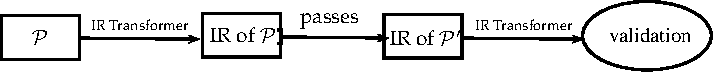
\includegraphics[width=.9\textwidth]{fig/se_workflow.pdf}
\bicaption[fig:se_workflow]{符号执行工具的整体工作流程}{符号执行工具的整体工作流程}{Fig}{Overall Workflow of a typical Symbolic Execution Tool}
\end{center}
\end{figure}

\section{KLEE简介}
\label{sec:llvm_klee}

\subsection{LLVM分析框架}
\label{sec:llvm}
LLVM的原意是底层虚拟机(Low Level Virtual Machine),是一个编译器基础框架,它提供了一种几乎和机器无关的中间表达形式(Intermediate Representation, IR或bitcode),使得任意程序语言只要可以表达成该形式都可以使用LLVM的分析框架进行优化。由于LLVM的中间表达形式将编译器前端和LLVM后端完整分离开来,只要满足LLVM的IR规约就可以生成正确的中间代码,这大大统一了分析的方法,降低了分析的门槛。同时,LLVM良好的设计使得在编译时期、链接时期、运行时期以及“闲置时期”都可以进行优化。符号执行引擎KLEE正是基于LLVM提供的这些特性才得以成为现实。越来越多的学者进行这方面的研究,基于LLVM的研究使得程序语言领域、软件工程方面取得的进展突飞猛进。

LLVM的中间表达形式语义极其丰富,可以支持ActionScript, Ada, D, Fortran, GLSL, Haskell, Java 字节码, Julia, Objective-C, Python, Ruby, Rust, Scala 和 C\#等多种语言。我们可以使用对应的前端工具如llvm-gcc,clang,dragonegg,llgo来使得生成对应的IR。LLVM提供了各种工具对这一中间表达形式进行分析、转化,如llvm-dis(中间代码反编译)/llvm-as(中间代码序列化),opt(中间代码优化)等;同时我们可以使用LLVM的API方便地编写LLVM的扩展应用,\dryrun 正是基于llvm的opt工具和其提供的分析、转化的API之上的。

\subsection{KLEE系统}
\label{sec:klee}

KLEE是建立在LLVM框架上的符号执行系统,出现于2008年,在2009年正式开源。具体说来,相比较以往的符号执行工具,KLEE有以下优势:
\begin{enumerate}
\item 对程序本身做了一些基于LLVM框架的编译优化(如常量传递、死代码消除等),简化待验证程序。
\item 结合了启发式路径探寻方法、约束集削减方法以及约束查找缓存机制,在很大程度上减少了约束求解器STP的查询次数。
\item 对内存进行了细粒度建模,利用了LLVM中间表达形式的扩展性,保证了程序执行状态的准确性。
\item 为了提高性能,它还利用了posix的底层fork机制,使得程序状态开销大大减少。
\item 提供了C的库函数$\mu clibc$的链接,使得通过一定的配置可以对文件、IO等底层函数符号化。
\end{enumerate}

KLEE的这些做法使得它适合处理偏向底层的程序,在对coreutils的89个工具测试中,在没有人工参与的情况下KLEE花费89小时生成的测试用例比15年来人工编写测试用例的覆盖率还高,同时找出了这些工具中被忽视多年的程序错误。这一结果使得人们意识到符号执行完全可以胜任特定系统环境下的测试用例集生成和错误检测。

\section{术语简介}
\label{sec:term}
为方便论述,首先介绍在\nameref{chap:symb}中提到的符号。
将原先的错误版本程序记为\bug ,而经过修改过的程序记为\patch ,一般意义下的程序使用\prog 来代指。如无特别说明,这3个符号的含义是宽泛的:既可以指代不加修改的源程序,也可以指代程序中的经过转化过的中间代码形式。

对于某一特定程序,将\prog 的出错位置(bug site)记为\prog\bs ,而把修改的补丁位置(可为多处)记为\prog\ps 。下面将会提到,\dryrun 所考虑的\prog\bs 都是程序中可能转化为断言的地方(assertion) \prog\ass ,故在源代码层次上,可以认为\prog\ass 和\prog\bs 都指的是assert宏的调用处(在C代码中一般会扩展为$\_\_assert\_fail$函数调用),后文将不加地区分使用这两者。\prog\bs 是导致程序执行时触发断言的根源程序片段,在实际中代指\bug 和\patch 中修改的代码对应的所在\bug 或\patch 中的那部分代码。和\prog\bs 不同,\prog\ps 可以为在代码上(源代码层次或中间层次)不连续的多个包含位置信息的代码片段(或仅为占位符性质的空操作)。若赋予程序中的语句以位置信息,在同一层次(可以是源代码或中间形式,也可以是经过若干步相同的优化后的代码)的转化下有等式\ref{eq:1}。
\begin{equation}
  \label{eq:1}
  (\bug \setminus \bug\ps )\cup \patch\ps = \patch
\end{equation}

程序的\rbscope 是\prog 的一个(非严格意义上的)子集,它包含了以指定的函数为执行入口,所有可能被执行到的程序相关代码片段。这样的\rbscope 有如下三种不同的精确程度:
\begin{enumerate}
\item 基于未被调用函数的削减结果。在指定了程序的入口函数之下,不少函数不会被调用到,在这种情况下可以首先剔除那些不会被调用的函数。这时的程序削减是依赖于调用图以函数为粒度的,得到的\rbscope 是\prog 的严格子集。
\item 基于基本块(Basic Block)可达性上的削减结果。该削减可能会额外添加含有不影响相关所关注路径语义的语句。
\item 基于对\prog\bs 影响性分析上的削减。同样,该削减会添加额外的语义以使得削减结果符合语法。
\end{enumerate}

对于某个程序\prog ,将其\rbscope 记为\prog\scope 。由于所做改动可能会导致数据流
和控制流及指向上较大的变化,\bug\scope 和\patch\scope 会有很大差异,并不能保证述等式\ref{eq:2}成立。
\begin{equation}
\label{eq:2}
(\bug\scope \setminus \bug\ps )\cup \patch\ps = \patch
\end{equation}

\section{一个典型例子}
\label{sec:gimp_example}

\autoref{fig:example} 展示了一段摘自GIMP 2.6.11\footnote{GIMP: GNU Image Manipulation Program, http://www.gimp.org/} Paint Shop Pro(PSP)插件简短的代码片段。图中以横线划去的部分为初始的不完整补丁,绿色的行为最终的正确补丁,而灰色的编辑行是通过\dryrun 的削减技术判断可以被删除的部分。当一个通过RLE压缩的PSP\_COMP\_RLE图像文件(第1行)在图像结束处{\tt runcount}(第7行)取值很大时,在第18行或者24行会发生基于堆的缓冲区溢出\footnote{https://bugzilla.gnome.org/show\_bug.cgi?id=639203.}。这一bug可能会被远程入侵者用于拒绝服务(DoS,denial of service)攻击,进一步可能被用于执行任意恶意代码。对该bug的第一个修改补丁位于第15行\footnote{https://abf.rosalinux.ru/fresh/gimp/blob/master/gimp-2.6.11-psp-overflow.patch}。然而该补丁是不完整的,它仅仅将第18行的bug修补了,第24行的断言仍然有可能被触发。这个问题于四个月之后第二次在CVE-2010-4543中被重新提出\footnote{http://web.nvd.nist.gov/view/vuln/detail?vulnId=CVE-2010-4543},最终有人给出了位于第16行的另一个补丁才终于将它修复。

如果程序员可以对第一次修改过的补丁程序进行验证,分析出\texttt{bytespp}和 \texttt{runcount}所有可能的取值,则可以避免这一不完全的补丁。然而,完全的补丁验证相对而言殊非易事(而对这一特例的补丁验证更为困难)。考虑到GIMP中有数百万的代码,普通的程序测试手段通常不能对该补丁进行完整测试,这是由于程序的规模增大导致了路径和程序状态以指数级增长。注意到第15行的程序相对较小,并且局限于修复第18行和第24行处的错误,如果将程序的关注范围局限于由补丁处至出错点处的部分,则可以大大减小待测程序片段的大小,因此可以对此使用规模相对较小然而更为完整的符号执行。我们给出了通过有选择性的符号执行来进行完整并快速的补丁验证的系统\dryrun 。

\begin{figure}[t]
\begin{center}
\begin{lstlisting}[language={[ANSI]C}]
%* \color{mygray}{case PSP\_COMP\_RLE: { } *)
  %* \color{mygray}{q = pixels[0] + offset;} *)
  %* \color{mygray}{endq = q + npixels * bytespp; } *)
  %* \color{mygray}{buf = g\_malloc (127); } *)
  while (q < endq) {
    %* \color{mygray}{p = buf; } *)
    fread (&runcount, 1, 1, f);
    if (runcount > 128) {
      runcount -= 128;
      %* \color{mygray}{{fread ($\&$byte, 1, 1, f); }} *)
      %* \color{mygray}{{memset (buf, byte, runcount); }} *)
    %* \color{mygray}{{\} else }} *)
      %* \color{mygray}{{fread (buf, runcount, 1, f); }} *)
      %* \color{mygray}{{/* prevent buffer overflow for bogus data*/ }} *)
      %* \sout{\texttt{runcount = MIN(runcount, endq - q);}} *)
      %* \color{mygreen}{\texttt{runcount = MIN(runcount, (endq-q)/bytespp);}} *)
      if (bytespp == 1) {
        assert (q + runcount < endq);
        %* \color{mygray}{{memmove (q, buf, runcount); }} *)
        q += runcount;
      } else {
        %* \color{mygray}{\texttt{p = buf;}} *)
        for (i = 0; i < runcount; i++) {
          assert (q < endq);
          %* \color{mygray}{{*q = *p++; }} *)
          q += bytespp;
        }
      } }
    %* \color{mygray}{{g\_free (buf); break; }} *)
\end{lstlisting}
\vspace{-0.5cm}
\bicaption[fig:example]{一个选择性符号执行的例子}{一个选择性符号执行的例子}{Fig}{An Illustrating Example for Selective Symbolic Execution}
\end{center}
\end{figure}


\section{\dryrun 的工作流}
\label{sec:dryrun_workflow}

\begin{figure}[t]
\begin{center}
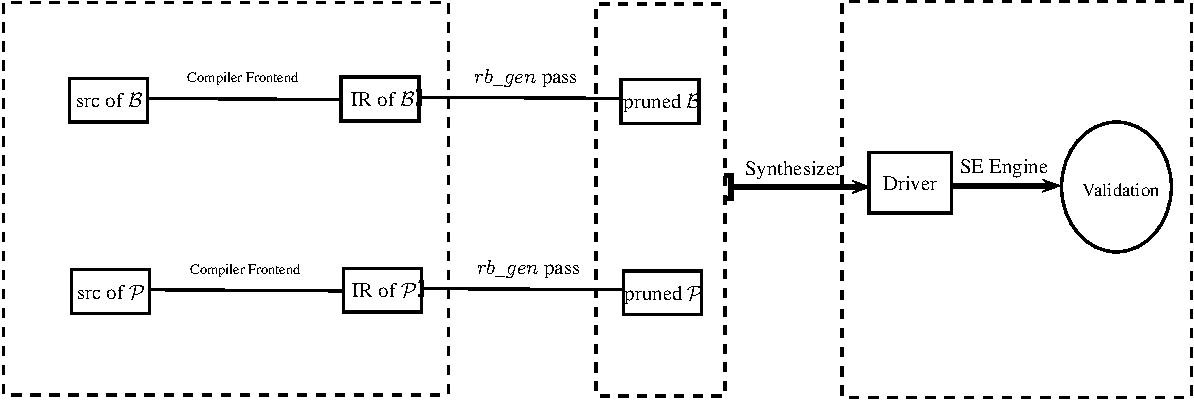
\includegraphics[width=\textwidth]{fig/workflow.pdf}
\bicaption[fig:workflow]{\dryrun 的整体工作流程}{\dryrun 的整体工作流程}{Fig}{Overall Workflow of \dryrun}
\end{center}
\end{figure}

\autoref{fig:workflow}展示了\dryrun 原理。和\autoref{fig:se_workflow}相比,不难看出\dryrun 的原创之处在于中间代码的转化上,并且使用两个版本程序经过添加程序驱动得以进行符号执行。

\noindent\textsf{定位程序\prog 的出错节点\prog\bs 和补丁节点\prog\ps\quad } 
\dryrun 首先根据源代码上的行号、变量名等信息确定程序配置程序的\prog\ps 及\prog\bs 。这里,\dryrun 主要关注的错误为程序中断言违反或可以转化为断言违反的缓冲区溢出或程序崩溃,对于C代码而言这是很常见的错误。另外,我们假设\prog\ps 是以差异(diff)文件为表现形式的,这可以从git、svn等源代码版本控制系统(version control system)管理的代码中非常方便地得到。因此,对程序\prog 的错误节点\prog\bs 及补丁节点\prog\ps 的定位是直接的:程序发生错误的节点所在语句被认为是\prog\bs,而修改(相对于原有的代码可能是添加、修改、删除一处或多处)的语句集合被认为是\prog\ps 。在\autoref{fig:example}这一例子中,第16行和第24行为\prog\bs ,而第15行为\prog\ps 。实际情形中,\prog\ps 和\prog\bs 都可能包含多个代码编辑行,在{\autoref{sec:complex}}将会提到如何对这一问题进行处理。

\noindent\textsf{程序中的极小有界区域的计算\quad} 
把\prog 的\prog\ps 和\prog\bs 作为输入,通过静态分析的方法,\dryrun 选取了补丁程序中的极小(minimal)部分(该部分即为\rbscope);这是通过三种不同粒度上的削减完成的。

首先依据上下文不敏感(context insensitive)的Andersen指向(points-to)算法,对程序的编译单元得到指向结果的概要(summary);在此基础之上,建立程序的精确调用图(call graph)信息,并得到函数调用点处(call site)处对变量的修改信息。至此,完成了基础的分析。之后,依据上述分析结果,对程序做未调用削减、基于可达性的削减及基于程序影响性分析的削减。

给定程序的入口函数,编译单元中存在一些未被调用的函数;这些函数虽然不会影响到最终的符号执行,但是会增加后期指向分析的复杂性,并且使得最终削减结果不够精确。基于此的削减是仅依赖程序的调用图信息。

对于由补丁处及错误处决定的程序片段,通过静态分析可以得到程序中的一些不可能被执行到的片段——这可以归结为程序的过程间控制流图(inter-procedural Control Flow Graph)的图可达性问题,将由程序补丁处不可达到的程序基本块(basic block)或不可到达程序出错处的基本块在保证关心路径语义正确的前提下进行削减。

程序的可达性分析并不能进一步削减程序中那些可达出错处但不会影响到该出错处的程序,对这些程序片段的削减是通过程序后向切片(backward slicing) (参见\ref{sec:slicing}) 完成的。涉及到的算法是基于不动点的,故最终削减结果并不唯一~\upcite{Slicing81};故而该有界区域是极小的而非最小。

\noindent{\textsf{生成验证驱动程序}\quad}
\dryrun 需要给\rbscope 添加上入口函数及符号执行的语义,使得可以被对应的符号执行引擎所理解。

对于上述例子\autoref{fig:example}的驱动程序,其结果如\autoref{fig:example_result}所示。其中合成器在第1至3行添加了变量的定义,并符号化未定义变量(第21行),同时程序员添加一些额外的前置条件(如第22行所示,具体参见\autoref{sec:user_init}), 进一步将\rbscope 封装在一个函数 $patch\_rbscope$中(第4至19行)。

\noindent{\textsf{基于符号执行的补丁验证}\quad} 
最终将所合成的驱动程序交由符号执行引擎进行执行。符号执行的分析工具保留当前的路径条件并由求解器计算出其所有可行结果条件,之后检测到程序出错路径是否可解。若路径可解,\dryrun 会警告这是一条不正确的路径;反之,认为该执行路径是正确的。

\noindent{\textsf{交叉验证}\quad}
为更进一步探究不正确的补丁程序是不完整的或引发了新的程序错误,\dryrun 还对原错误程序及补丁程序的执行作了比较。这一过程需要将两个版本的程序同时融合于一个编译单元中,并向原有的程序驱动中添加交叉验证的操作语义。这使得可以在更精确的路径粒度上对不同版本程序进行分析。

\begin{figure}[t]
\begin{center}
\begin{lstlisting}[ basicstyle=\ttfamily\bfseries\footnotesize, language={[ANSI]C}]
char *buf, *q, *endq;
unsigned int bytespp, runcount;
FILE *f;
patch_rbscope() {
  while (q < endq) {
    fread(&runcount, 1, 1, f);
    if (roncount > 128)
      runcount -= 128;
    runcount = MIN(runcount, (endq-q)/bytespp);
    if (bytespp == 1) {
      assert (q + runcount < endq);
      q += runcount;
    } else {
      for (int i = 0; i < runcount; i++) {
        assert (q < endq);
        q += bytespp;
      }
    } }
}

int main(void) {
  make_symbolic(&q, &endq, &bytespp, &f);
  assume(q < endq);
  patch_rbscope();
}
\end{lstlisting}
\vspace{-0.5cm}
\bicaption[fig:example_result]{对\autoref{fig:example} 生成的驱动程序}{对\autoref{fig:example} 生成的驱动程序}{Fig}{Generated driver program for \autoref{fig:example}}
\end{center}
\end{figure}

\section{本章小结}
\label{sec:c2}
本节主要介绍了\dryrun 所使用的选择性符号执行中涉及到的一些技术。首先介绍了符号执行的基本概念,并分析了影响符号执行扩展性的几个挑战;接下来简单介绍了\dryrun 所基于的LLVM框架及符号执行工具KLEE。在给出了\nameref{chap:symb}中符号的表示意义之后,通过一个具体的例子,解释\dryrun 的具体工作流程。
\chapter{\rbscope 的生成}
\label{chap:impl}

本章将详细讨论\dryrun 实现中使用到的\rbscope 生成的一些技术,这部分主要是\dryrun 的第一部分,主要是通过静态分析的方法对给定程序进行无关语句削减。

由于\dryrun 是在LLVM的中间表达形式上实现的转化(LLVM的中间表达形式的特点参见\autoref{chap:IR}),故如无特别说明,下文涉及到的程序的转化都是在LLVM的IR上完成的;由于LLVM的中间形式较为底层并且不易理解,后文采用与之等价的C语言代码来表述。

\section{生成\rbscope 的流程 }
\label{sec:rb_gen}
生成\rbscope 时的流程依赖图如\autoref{fig:rb-gen}所示,其中图中的实线箭头表示流程间的直接依赖关系,虚线箭头表明该依赖关系是可选的;加粗边框的椭圆是可作为最终结果的流程。从图中可以看出,对某一编译单元的分析是精确的指向分析的。
\begin{itemize}
\item 在指向分析的基础上,构建调用图信息。
\item 由于 \autoref{sec:complex} 提及的原因,复杂的关注点可能需要调用图信息来得到其\prog\ps 信息。
\item 在给定指向分析和调用图信息及关注点配置的前提下,削减程序中未被调用的函数。
\item 基于未调用函数削减、关注点配置及调用图完成可达性分析并基于此对程序进行削减。
\item 依赖指向分析、未调用函数削减、关注点配置及调用图信息,进行过程间程序切片;这一过程可以在可达性的削减上进行,也可以在未调用函数削减的基础上进行。
\end{itemize}
上述过程中每一次程序的转化都需要重新建立过程间的分析。

\begin{figure}[t]
\begin{center}
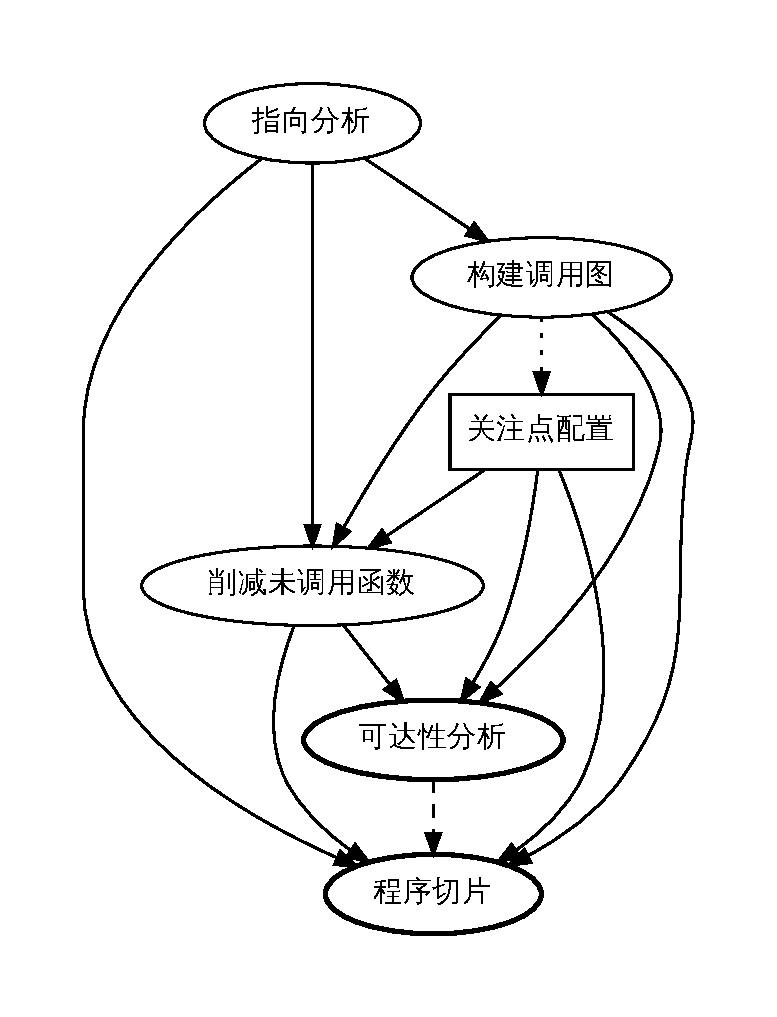
\includegraphics[width=.6\textwidth]{fig/rb_gen.pdf}
\vspace{-24pt}
\bicaption[fig:rb-gen]{生成\rbscope 的流程图}{生成\rbscope 的流程图}{Fig}{Flowchart of \rbscope{} Generation}
\end{center}
\end{figure}

需要说明的是,出于符号执行的需要,通过程序削减生成\rbscope 的过程需遵循下面的基本原则:
\begin{enumerate}
\item 保留下的程序必须包含所有可能执行的代码,即削减过程必须是保守(conservative)的。
\item 保留下的程序在添加了驱动程序之后必须是可执行的。
\item 出于选择性符号执行要求,削减程序过程应该尽可能精确。
\end{enumerate}


\section{关注点配置}
\label{sec:config}
\dryrun 以C语言为主要研究对象,需要在源代码层次上指定关注点及入口函数信息,并反映到中间表达形式上。因为编译预处理、编译、链接及中间形式优化等原因,由C语言语句到LLVM中间形式指令的映射既非单射也非满射,在不修改LLVM前端的情况下并没有通用的方法在中间表达形式上准确定位源代码层次的特定位置处变量信息(但入口函数可以通过函数名配置)。由于\rbscope 需要\prog\ps 和\prog\bs 的信息,故至少这两者需要从外界接收。

出于程序除错的需求,目前仅将关注点局限于C语言中的assert宏中的条件变量, 在 LLVM的IR层次需定位特定的$\_\_assert\_fail$(由assert宏扩展而来)调用点,找到其所有前驱基本块的终结指令中的条件变量。一般而言程序中的assert调用不止一处,需要根据程序的debug信息来定位所关心的断言调用处。这一定位操作可细化为: 
\begin{enumerate}[label={(\arabic*)}]
\item 由源文件的配置信息在中间表达形式层添加元数据。
\item 由元数据解析得到中间形式下的关注点信息。
\end{enumerate}

扩展现有切片准则情形(即不限于assert的宏调用)有如下两种解决方案:
\begin{itemize}
\item 通过源代码层次的重构,使得待处理程序是经规范化的、更接近LLVM中间表达形式的“标准型”;可通过 openrefactory\footnote{http://openrefactory.org/}等C语言重构工具来实现。
\item 在源代码上添加注释,修改C语言的LLVM前端抽象语法树构建过程,由clang生成(1)中的元数据。
\end{itemize}

\subsection{入口函数配置}
\label{sec:entry_config}
这里显式要求使用者自行提供入口函数的信息,因为即使是在函数层次上,依据\prog\ps 和\prog\bs 仍然无法给出程序可能的执行路径。如下面的例子中,\prog\ps 为第4行,而\prog\bs 为第7行,但是以foo或bar为函数入口都可以包含\prog\ps 和\prog\bs 。因此,若仅由\prog\ps 和\prog\bs 来求解入口函数,应当使用算法\autoref{alg:entry}中的方法。

\begin{figure}[t]
\begin{center}
\begin{lstlisting}[language={[ANSI]C}]
void patch_fn(int *p) { 
  *p = (*p > 0) ? (*p) : (-*p); 
  // patch site
  // *p = *p + 1;
}

void bug_fn(int i) { assert(i > 0); }

void foo(void){
  int i = 0;
  patch_fn(&i);
  bug_fn(i);
}

void bar(void) {
  int i = 1;
  patch_fn(&i);
  bug_fn(i);
  foo();
}
\end{lstlisting}
\bicaption[fig:entry]{入口函数的配置举例}{入口函数的配置举例}{Fig}{An Example for Entry Function Configuration}
\end{center}
\end{figure}

\begin{algorithm}\label{alg:entry}
\caption{入口函数定位算法}
\SetAlgoNoLine
将直接包含 \prog\ps 的函数标记为 $\mathcal{F}{_{pfn}}$, 直接包含 \prog\ps 的函数标记为 $\mathcal{F}{_{pfn}}$

根据调用图,计算得到所有直接或通过函数指针间接调用 $\mathcal{F}{_{pfn}}$ 的函数集合$\mathcal{F}_{p}$; 计算可以调用$\mathcal{F}_{p}$所有函数的闭包,记为$\widehat{\mathcal{F}_{p}}$

根据调用图,计算得到所有直接或通过函数指针间接调用 $\mathcal{F}{_{bfn}}$ 的函数集合$\mathcal{F}_{b}$; 计算可以调用$\mathcal{F}_{b}$所有函数的闭包,记为$\widehat{\mathcal{F}_{b}}$

计算$\widehat{\mathcal{F}_{p}}$ 和$\widehat{\mathcal{F}_{b}}$的共同主调函数,将之作为入口函数\prog\entry
\end{algorithm}

对于上述例子,采用这样的算法得到的入口函数是bar;然而存在处于某种原因可以说明bar中由函数bug\_fn调用的断言一定为真而不需要额外验证的情形,故只需将入口函数限制于foo上。在\dryrun 实现中,允许用户指定入口函数,当没有提供入口函数时,使用上述算法得到的函数进行配置。若为手动配置,需要用户来保证从入口函数出发一定会执行到\prog\ps 和\prog\ass 。

\subsection{复杂补丁处理}
\label{sec:complex}
\autoref{fig:example} 的程序中仅涉及到了补丁对原有程序\bug\ps 一处的修改操作,且并不包含复杂的数据结构。现实中的补丁往往还包含添加、删减等改变,并且其改动不限于一处。为处理复杂补丁,\dryrun 将程序的改动看作是给定相对位置信息的语句集合和空语句之并。在程序差异(diff)文件上来看这是直接的:修改语句被另一语句所替代,给添加的语句补丁的\bug 版本添加一条在\patch 中对应位置处的空语句,删除语句的补丁类似。 \autoref{sec:entry_config} 给出的配置规约可以保证所给的补丁部分都被包含到了\rbscope 中,故可将补丁的讨论限制在由配置信息确定的\prog\scope 中。对于复杂补丁处理的基本思路仍然是将之化归到单一修改的补丁问题上。

对于\prog\ps ,所有的分析是在基本块层次上的;这是因为基于语句(指令)的分析会遇到如下困难:
\begin{enumerate}
  \item 由于代码转化是在LLVM的中间表达形式层面的,其表达形式无法与源代码中的语句一一对应。尤其是遇到源代码中以聚合类型(如数组、结构体等)的某个元素或域为关注点,在中间表达形式中没有相应的域,故将\prog\ps 细化到变量层次上是不可行的。
  \item 对于添加、删除语句类型补丁,对于语句较少版本的程序,使用的是空语句来作为补丁节点,由于数据流、控制流等分析结果,无法得到影响到\prog\bs 的语句。
  \item 补丁语句分布于多个函数中时(参见算法\autoref{alg:complex}),没高效准确的算法可以将补丁位置精化到语句或变量层次。
  \item 削减中基于\prog\ps 的削减仅在可达性分析上使用,这是建立在基本块上的;故没有必要精确到语句层次。
\end{enumerate}

算法由算法\autoref{alg:complex} 给出。
\begin{algorithm}\label{alg:complex}
  \caption{复杂补丁配置}
  \SetAlgoNoLine
  记$\prog\ps = \{p_1, p_2, \cdots , p_n\}$, 以基于基本块的可达性(\autoref{sec:reach})为基准划分为等价类$\prog _{ps}=\{P_1, P_2, \cdots , P_m\}$ ,其中$P_j(j\in\{1, 2, \cdots , m\})$的代表元素为所有可以到达等价类中其他元素的基本块(即在执行过程中它“首先”被执行到,至少存在一个这样的基本块)。若$m=1$,则选取$P_1$作为补丁,算法终止。

以$\prog_{ps}$中各元素所在基本块$BB_j$为单位,在各自所在的函数内求解$Dominator_k$($k\in\{1, 2, \cdots , s\}$)(基本块)。若$s=1$,则选取$Dominator_1$作为补丁,算法终止。

计算$Dominator_k$($k\in\{1, 2, \cdots , s\}$)所在函数的直接主调函数(caller)的调用点所在基本块$BB_l$($l\in{1, 2, \cdots , t}$),计算可以到达其他基本块的元素作为补丁。
\end{algorithm}

需要说明的是,该算法仅使用于函数本身不包含程序控制流图修改的补丁改动。

\section{指向分析}
\label{sec:andersen}

\subsection{基本概念}
\label{subsec:pt_basic}

指向分析是一种建立指针类型变量和它可以指向的变量地址之间关系的分析。指向分析可以进一步细分为:
\begin{itemize}
\item 域(不)敏感(field sensitive/insensitive):是否区分结构体变量的域而把指向作为结构体变量本身。
\item 上下文(不)敏感(context sensitive/insensitive):是否区分函数调用点的上下文而只关心程序退出时的指向情况。
\item 流(不)敏感(flow sensitive/insensitive):是否区分控制流而对可能指向的集合取并操作。
\end{itemize}
精确的指向分析的开销很大,实际情况下指针分析的扩展性较差,广泛使用的是上下文不敏感和流不敏感的Andersen算法~\upcite{Andersen94programanalysis}和Steensgaard~\upcite{Steensgaard1996}算法。前者基于子集的指向集求解,更为精确;后者基于类型系统上的等价类划分,时间复杂度低。

\subsection{Andersen算法}
\label{subsec:andersen}
选取了流不敏感、上下文不敏感的指向分析中最为精确的Andersen~\upcite{Andersen94programanalysis}算法,对现有的points-to实现做了改动。上下文不敏感的Andersen算法仅相当于得到函数退出前指向关系的概要而非程序关注点处的结果,这会导致削减不够精确。如\autoref{fig:andersen}中,当程序关注点为“$assert(j > 0);$”时,$p$应该仅可能指向$j$,然而由于指向分析是流不敏感的,故仍然会认为可能指向$i, j$或$k$。当涉及类似于C语言中的函数指针时会保留更多的不相关分支。

\begin{figure}[t]
\begin{center}
\begin{lstlisting}[language={[ANSI]C}]
  void foo(void) {
    int a, i, j, k;
    int *p;
    if (a < 0) {
      p = &i;
      *p = 3;
    } else if (a > 0) {
      p = &j;
      *p = 3;
      assert(j > 0); // <= interest point
    }
    p = &k;
    *p = 3;
  }
\end{lstlisting}
\bicaption[fig:andersen]{流不敏感的Andersen带来的问题}{流不敏感的Andersen带来的问题}{Fig}{Issues about Flow-Insensitive Andersen Algorithm}
\end{center}
\end{figure}

\section{调用图的建立}
\label{sec:callgraph}

\subsection{基本概念}
\label{subsec:cg_basic}
调用图是一种表征主调函数和被调函数之间关系的有向多图(directed multi-graph)。 对于同一个程序,不同的程序输入会带来不同的调用图;例如gprof根据每次动态执行的结果得到对应的调用图。对静态分析而言,在给定了程序的起始执行函数之后,需要建立一个包含所有可能的被调函数的调用关系。由于间接调用的存在,不同精度的指针分析结果同样会得到不同的调用图。

\subsection{调用图的实现}
\label{subsec:cg_impl}

LLVM选用“使用定义对”构建调用图,这样的结果是粗糙的。\autoref{fig:callgraph}是一个说明了该问题的例子。
\begin{figure}[t]
\begin{center}
\begin{lstlisting}[language={[ANSI]C}]
int dec(int i) { return i - 1; }

unsigned long func1(int i) {
  if (i == 0) return 1;
  return func1(dec(i)) * i;
}

unsigned long func2(int i) { return i * 0; }

unsigned long (*pF)(int) = func1;

int getNextRandomValue(void) { 
  return rand() % 10; 
}

void populate_array(int *array, size_t arraySize, int (*getNextValue)(void)) {
  for (unsigned i = 0; i < arraySize; i++)
   array[i] = getNextValue();
}

int main(void) {
  int i = 3;
  int myarray[10];
  if (i < 3) {
    pF = func1;
  } else {
    pF = func2;
  }
  pF(getNextRandomValue());
  populate_array(myarray, 10,  getNextRandomValue);
}
\end{lstlisting}
\bicaption[fig:callgraph]{调用图的例子}{调用图的例子}{Fig}{An Example about Call Graph}
\end{center}
\end{figure}

上述执行当中,从main出发,在条件分支上存在函数指针的赋值,而之后有对应的函数调用,在没有常量传递等编译器优化的情形下,需要将func1和func2都作为main函数的直接被调用函数。另一方面,populate\_array采用指针传递的方式调用了getNextRandomValue;准确的调用图如\autoref{fig:accurate_cg}所示。LLVM的基本调用图参见\autoref{fig:llvm_cg}:

准确的调用图算法实现如算法\ref{alg:callgraph}所示。
\begin{algorithm}\label{alg:callgraph}
\caption{准确调用图的生成}
\SetAlgoNoLine
遍历整个编译单元,当遇到调用点,转至step2

若该调用处的值为函数常量,则将该主调函数和被调函数对加入直接调用的directCaller2CalleeMap中;若该调用点为间接调用,通过指向分析找出该变量所指向的所有可能的值,将主调函数和这些值结对加到directCaller2CalleeMap中。记录被调函数和调用点信息于directCallee2CSMap中。

重复上述两步直至遍历完成。将所有的直接调用的caller到callee的映射(directCaller2CalleeMap)传递给间接调用的caller到callee的映射(Caller2CalleeMap)。
\end{algorithm}

\begin{figure*}[!t]
\centering
\subfigure[LLVM's Basic Call Graph]{\label{fig:llvm_cg}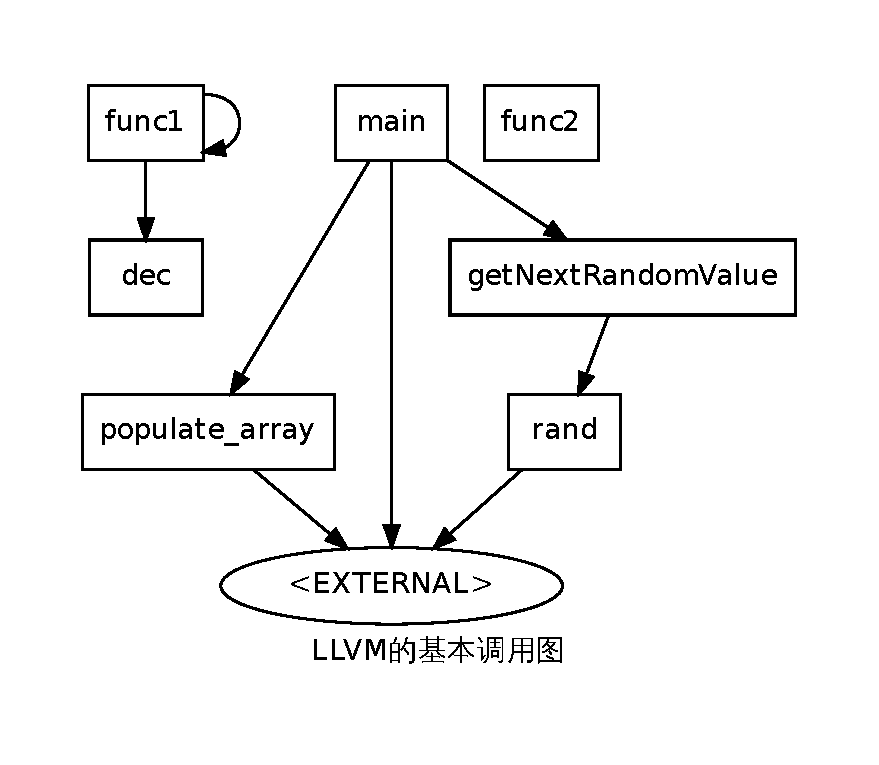
\includegraphics[width=.6\textwidth]{fig/cg_llvm.pdf}}
\hspace{1in}
\subfigure[Accurate Call Graph]{\label{fig:accurate_cg}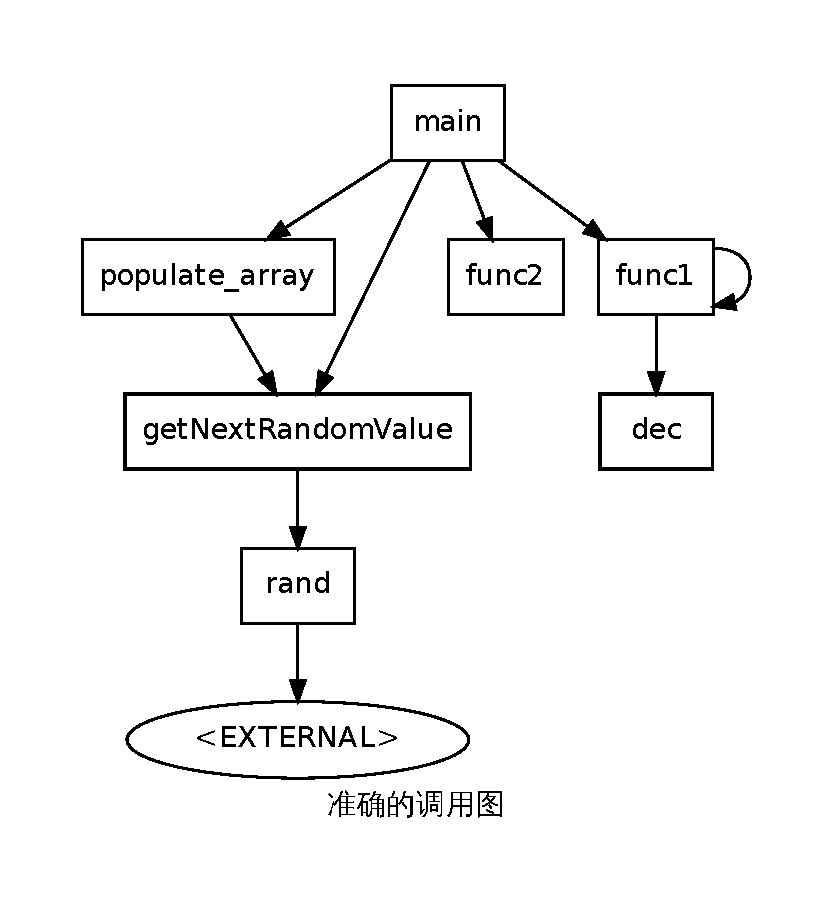
\includegraphics[width=.6\textwidth]{fig/cg.pdf}}
\bicaption[fig:callgraphs]{调用图比较}{调用图比较}{Fig}{Comparison of Call Graphs}
\end{figure*}

经过该算法得到的调用图仍然会存在外部节点,这是因为部分函数没有定义而只有声明,无法判断其调用信息。对于一个可执行程序,这样的函数来自于:
\begin{enumerate}[label={(\arabic*)}]
\item 外部库函数
\item 未使用的函数声明(例如头文件的函数声明)
\end{enumerate}
若为情形(1),可以保证该库函数不会调用任何一个在该编译单元中的函数;对于情形(2),这类函数可通过\autoref{sec:uncalled}中的方法消除。

\section{基于未被调用函数的削减}
\label{sec:uncalled}

对已建立的函数调用图,给定程序的入口函数(如main函数)仍可做一些额外的削减。这是因为在同一个编译单元里的函数有可能不会被调用(即在调用图上,从入口函数到该函数之间没有路径)。步骤如下:
\begin{algorithm}\label{alg:uncalled}
\caption{未被调用函数的削减}
\SetAlgoNoLine
遍历编译单元中的函数表,若该函数不在Caller2CalleeMapentry中,将该函数的函数体置空,并标记为待删除函数。

遍历待删除函数集合,逐一从编译单元中删除。
\end{algorithm}

该过程同时解决了\autoref{subsec:cg_impl}中的外部节点的情形(2)所带来的外部节点问题。本操作的必要性将在\autoref{sec:inter-reach}提及。

\section{基于可达性的削减}
\label{sec:reach}

\subsection{过程内分析}
\label{subsec:intra-reach}

过程内的可达性分析将函数调用点看作普通节点。LLVM的中间表示形式中的每个函数以基本块划分为不同的节点,且可以保证单一的入口;同时可以通过PHI函数合并使得仅有一个return语句。考虑函数中任意基本块是否可以执行到某一特定基本块(语句或指令层的可达性可以由基本块迅速导出),该问题退化为一般的图可达性问题,通过经典的DFS/BFS算法实现。\autoref{sec:inter-reach} 的分析说明不能将过程内的不可达分析用于削减。

\subsection{过程间可达性}
\label{sec:inter-reach}

由于所关注的语句所在函数可能被调用多次,在同一函数内对同一条语句(或指令)过程内可达集合是过程间可达的子集。以下述程序为例说明其差异性。

\begin{figure}[t]
\begin{center}
\begin{lstlisting}[language={[ANSI]C}]
int foo(int i) {
  if (i < 0) {   
/// interest point
    return -i;
  } else {
    return i;
  }
}

int foo1(int i) { return foo(i); }

int foo2(int i) { return foo(i); }

int main(void) {
  int i = -1;
  foo2(-i);
  foo(i);
  return 0;
}
\end{lstlisting}
\bicaption[fig:reach]{可达性分析典型例子}{可达性分析典型例子}{Fig}{A Classic Example about Program Reachability}
\end{center}
\end{figure}
以foo函数中的if分支的return语句作为关注点,在分析过程内可达性时,else分支不可以通过任何路径达到该点。然而在过程间分析时,由于foo2调用了foo之后foo又被main函数直接调用,静态分析需保守认为存在一条在foo2调用foo时执行了else分支、而foo执行了if分支,故在过程间分析中else分支的语句需被计入可达关注点的集合中。 另一方面,foo1中的调用函数foo的语句可以达到关注点,然而因为foo1没有被入口函数调用(这里为main),故不可达关注点,这正是\autoref{sec:uncalled}削减未调用函数的原因。

不同于过程内的可达性分析,过程间的分析必须关注函数调用点——在函数调用前后的可达性是截然不同的。这需要我们特殊对待基本块中的调用点前后。其实现参见算法\ref{alg:reach}。

\begin{algorithm}\label{alg:reach}
\caption{可达性算法}
\SetAlgoNoLine

将每个基本块以函数调用点为界限划分为多个“子基本块”。初始认为仅关注点所在子基本块可达。

(1)在过程内计算可达性,更新该子基本块为可达。(2)将可达调用点的所有未完全被访问(函数中至少存在一个调用点未被访问)的被调函数及该被调函数的所有未完全被访问的callee(Caller2CalleeMap)的所有基本块都更新为可达,标记所有的callee的所有调用点为已访问。

根据directCallee2CSMap得到关注点所在函数的所有未被访问的被调用点(采用队列的方式)。
将每个被调用点作为间接关注点,标记重复step2,step3中的操作直至(1)所有函数中的调用点都被访问过。
\end{algorithm}

需要注意的是,这里不考虑特殊的函数调用会影响可达性结果:例如exit()函数调用处于某个基本块中间;或setjmp/longjmp函数调用等。

\subsection{基于可达性的削减}
\label{subsec:reach-prune}

并非所有的不可达语句均可削减,这是因为不适当的削减会导致程序不可执行,而错误的基本块拼接会影响到关注点的执行路径。实现时将这些分支的内容转换成立即退出的特殊函数调用:
\begin{algorithm}\label{alg:reach-prune}
\caption{基于可达性的削减}
\SetAlgoNoLine
对编译单元中的每一个基本块(或子基本块)计算其到关注点的可达性,将不可达节点放入不可达集合中,并将不可达节点所在的终结指令替换成LLVM中的不可达指令。

遍历不可达集合中的基本块(或子基本块中所在基本块):若未被用,则将该块内容置空,并将该块从编译单元中删除;若其仍被使用,则将该块内容替换成exit(1)的函数调用。
\end{algorithm}


\section{基于程序影响性分析的削减}
\label{sec:slicing}

程序切片比基于可达性的削减更为精确,后者的削减结果是仅包含实际可执行至关注点的语句,而前者进一步剔除那些可达到关注点、但并不影响关注点结果的语句。类似于可达性分析,程序切片过程间的分析集合比过程内的分析更为保守安全;与可达性分析不同,这里的分析完全应用于LLVM的指令层次。过程间分析采用了Mark Weiser提出的基于控制流图的过程内分析和过程间调用点传递的方式~\upcite{Slicing81}。
% \todo{add algo}

细节上有如下改变:
\begin{enumerate}
\item 由于部分LLVM的IR中的指令的结果值本身为变量(如LoadInst/CastInst或返回值的CallInst等),在实现过程中不严格区分语句和变量而只关心指令和其操作数。对每一读写内存操作,考虑其可能的指针变量的指向集合,并在函数的调用处分析其修改变量信息。
\item 经典切片算法中不涉及程序Load/Store这类内存相关指令,为此首先使用了LLVM的mem2reg这一转换,消除了程序中不必要的内存读写指令。同时将Store操作的指令所写地址既作为定义(DEF)又作为使用(REF),这是因为LLVM既对所写地址变量直接操作(类似于地址运算),又可以对地址处的内容所存放值运算(通过Load)。对其他切片算法中没有的指令类型,采用类似的手段进行模拟。
\item LLVM的IR要求每个基本块必须以终结指令结束,故(3)中必须保留分支跳转语句、switch语句等。然而存在跳转的条件变量为undef的削减结果,这对应该分支为不相关分支的情形,可以通过LLVM的PHI函数解决。
\end{enumerate}
这是一个不动点的算法,每一次相关集的改变都需要重新修改甚至整个编译单元的相关集,代价是巨大的。将\autoref{sec:reach}中的过程间可达性算法与之结合,可以在实际中大大削减分析开销。

经过程序切片得到的\rbscope 是仅由程序可达性分析得到的\rbscope 的一个精化。直观而言,它包含的语句在执行时可能生成的路径需满足:
\begin{itemize}
\item 连接了\prog\ps 和\prog\bs
\item 对程序中的断言\prog\ass 上的条件值有影响
\end{itemize}

这里没有使用forward slicing用来计算\prog\ps 影响到的程序片段,其原因参见\autoref{chap:fwd_issue}。

\section{本章小结}
\label{sec:c3}

本章具体阐述了\rbscope 的生成算法。首先给出了\rbscope 的生成流程图,对其依赖关系作了解释。接着,对\rbscope 生成中的每个步骤进行了详尽的说明,分别是\nameref{sec:config}、\nameref{sec:andersen}、\nameref{sec:callgraph}、\nameref{sec:uncalled}、\nameref{sec:reach}、\nameref{sec:slicing},对于没有经典实现的分析或转化算法给出了其在LLVM中间代码上的具体实现。
\chapter{补丁验证}
\label{chap:linker}

上一章说明了产生\rbscope 的过程,本章将详述根据生成的\rbscope 进行补丁验证的方法。

\section{单程序的补丁验证}
\label{sec:validate}
对于一个由程序的配置信息和静态削减得到的\rbscope ,需要添加一些额外的符号执行语义及驱动程序代码才可以被符号执行引擎所使用。算法\ref{alg:validate} 给出了它的算法。
\begin{algorithm}\label{alg:validate}
\caption{单程序的补丁验证}
\SetAlgoNoLine

将原本属于本编译单元的全局变量通过符号化函数$klee\_make\_symbolic$转化为“符号变量”。

为\prog\entry 中的函数参数在编译单元模块上分配存储空间(类似于全局变量)。根据变量的类型信息,将这些全局变量转化为“符号变量”。

将函数中所关注的\prog\ass 转化为条件分支语句$if\cdots else$的形式,当满足assert被触发的条件时对应的标记位为1。

给编译单元添加main函数(若入口函数本身为main函数则需将之重命名以示区别),将上述转化而来的“符号变量”以实参形式带入函数中。

根据最弱前置条件给符号化的变量通过$klee\_assume$接口添加前置条件。

使用KLEE对新生成的编译单元进行符号执行,从得到的符号执行结果中得到该\rbscope 对应的原有程序的正确性。
\end{algorithm}

\section{交叉验证}
\label{sec:cross}

若存在一个输入值使得程序同时触发了bug版本程序\bug 和patch版本程序\patch 所在关注点处的断言\bug\ass 和\patch\ass,则该补丁程序是不完整的。若存在一个输入值使得断言\patch\ass 被触发而对于任意一个给定输入\pin 都没有触发 \bug\ass ,则称一个补丁是一个回归补丁(regression patch)。通常,一个不正确的补丁\patch\ps 可能是不完整的、回归的或两者兼而有之。若不对\bug 和\patch 结果进行比较,我们无法进一步区分\patch\ps 是否为回归的或是不完整的。

因此,类似于对\patch 的做法,\dryrun 对\bug 同时进行有选择性的符号执行;在编译单元的生成中,采用了\autoref{fig:cross_valid}中的做法。函数\textmd{buggyRB} 和 \textmd{patchBB} 分别是\bug 和\patch 对\rbscope 的封装后的函数(这是为了方便说明问题假想的函数,后文将叙述其实现;在这里可简单认为是包含\prog\ps ,\prog\bs 的入口函数\prog\entry )。在这里,程序\prog 中原有的\prog\ass 被替换为对应的条件分支语句;在符号执行时如果对应于buggyRB(或patchBB)中原有断言被触发的分支,则将对应的标志位\textmd{error\_bug} (或\textmd{error\_patch})置为True。而函数\textmd{corss\_validate} 则用于检测补丁程序是否是不完整(第3、4两行)的或包含回归错误(第7、8两行)。这一基于执行的比较需要两个版本程序的输入值是相同的,即符号变量参数\textmd{symargs}的约束条件是一致的。因此,需要将调用\textmd{patchBB} 的调用点放置于\textmd{error\_bug} 被设置的程序处。注意到这里需要满足的一个条件为对符号变量的本身没有修改操作(即程序的副作用对符号变量没有影响),一般而言这需要静态单赋值(static single assignment)的支持,这在LLVM的中间代码表达形式上可以局部支持;而对于符号变量在原完整程序\prog 编译单元中即为全局变量并在\prog\ps 和\prog\bs 这种情形,目前仍是通过实现将程序“规范化”的方法来完成的。最终,\textmd{cross\_validate} 在\textmd{patchBB} 函数退出前被调用。需要指出的是,程序的调用方式可以反过来,即\textmd{patchBB} 亦可以在\textmd{main} 函数中被调用,而\textmd{buggyBB} 则在\textmd{patchBB} 中被调用并且\textmd{cross\_validate} 在\textmd{buggyBB} 中被调用。

为了进行交叉验证,目前的实现上\dryrun 需要对两个版本的程序分别计算出\rbscope ;之后交给\dryrun 提供的链接器rb\_link 来进行转换。
\begin{itemize}
  \item 把\bug\scope 和\patch\scope 中共有全局变量转化为符号值,并给\bug\entry (或\patch\entry )的形式参数分配类型相容的空间,符号化该存储内容。
  \item 在main函数中调用\bug\entry ,其实参为经过符号化之后的函数形参变量。
  \item 在添加标志位$error\_bug$和$error\_patch$,并添加$cross\_validate$的函数定义(见\autoref{fig:cross_valid}的$cross\_validate$函数)。
  \item 将\bug\ass 和\patch\ass 转化为对应的分支结构,并在当原有条件会触发assert断言时,修改相应的标志位。例如在\bug\ass 所在的函数中,若在源代码层次上的\bug\ass 为$assert(cond);$的情形,则在$cond$成立的分支上添加$error\_bug=1;$,对于\patch\ass 情况类似。同时在\patch\ass 的每个分支上调用$cross\_validate$,在\bug\ass 的每个分支上调用$\bug\entry$。
\end{itemize}
  
另一方面,当得到的结论是补丁程序是不完整时,可以分析符号执行结束后生成的测试用例来判断相对于\bug 而言,\patch 版本仍然会触发错误的路径和\bug 触发错误的路径数量进行比较以评价补丁程序。

\begin{figure}[t]
\begin{center}
\begin{lstlisting}[language={[ANSI]C}]
/*------- cross validate part ------- */
  int patch_error = 0, bug_error = 0;
  void cross_validate() {
    if (bug_error && patch_error)
      assert(0, "incomplete patch!");
    else if (bug_error && !patch_error)
      assert(0, "bug fixed!");
    else if (!bug_error && patch_error)
      assert(0, "regression patch!");
    else
      assert(0, "correct and no change!");
  }

/*-------  the driver part ------- */
  void patchedRB() {
    { // the rbscope of patched program
      ...
      patch_error = 1; // replace patch program assert
    }
    cross_Validate();
  }

   void buggyRB(void) {
    { // the rbscope of buggy program
      ...
      bug_error = 1; // replace bug program assert
      patchedRB();
    }
  }

  int main(void) {
    make_symbolic(symargs);
    buggyRB();
  }

\end{lstlisting}
\vspace{-0.5cm}
\bicaption[fig:cross_valid]{交叉验证在源代码上的伪代码表示}{交叉验证在源代码上的伪代码表示}{Fig}{Pseudo Code Representation for Cross Validation at Souce Code Level}
\end{center}
\end{figure}

\section{用户提供的上下文初始化}
\label{sec:user_init}

对于一些有很多符号变量的复杂结构的\rbscope , 单纯使用上述的符号化未知值变量的方法仍然可能使得符号执行时间很长。因此,\dryrun 允许用户做一些简单的变量的具体化\cndash 提供具体的输入值而不是完全使用符号值, 从而减少符号执行的状态空间。这些上下文初始化包括:使用合适的变量值创建并初始化复杂数据结构, 适当减少需要符号化的变量, 并尽可能给出入口函数处程序的最弱前置条件。
以来自于Coreutils中的tsort.c这一代码作为例子,函数\texttt{search\_item(struct item *root, const char *str)}的作用为在以根节点为\texttt{\textmd{root}}的平衡二叉树中寻找字符串\texttt{\textmd{str}},其返回值或者返回匹配\texttt{\textmd{str}}的节点,或者将\texttt{\textmd{str}}插入到该二叉树中。其中涉及到平衡属性的程序断言来验证程序实现的正确性。

在这种情况下,将这个二叉树进行符号执行会导致一种情形:程序不断插入新的节点而使得该程序执行路径无法终止,这是没有意义的。在这种情况下,用户需要提供上下文来初始化一个具体的平衡二叉树,而仅仅将节点内容作为符号值在\texttt{\textmd{Context\_Init}} 中初始化,并且在\texttt{\textmd{Context\_Finalize}} 做结束工作。最终\dryrun 将他们封装在一起,其结果的伪代码参见图~\ref{fig:init}。

\begin{figure}[t]
\begin{center}
\begin{lstlisting}[language={[ANSI]C}]
static struct item *search_item
    (struct item *root, const char *str);

int Context_Init() {
  Init_BBST(root);
}

int Context_finalize() {
  Finalize(root);
}

int main(void) {
  char str[2];
  make_symbolic(str, 2, "s_root_str");
  assume(str[1] == '\0');
  struct item *root;
  Context_Init();
  search_item_rbscope(root, str);
  Context_Finalize();
}
\end{lstlisting}
\vspace{-0.5cm}
\bicaption[fig:init]{一个包含用户具体化上下文的例子}{一个包含用户具体化上下文的例子}{Fig}{An Example about User Provided Context Initialization}
\end{center}
\end{figure}


\section{本章小结}
\label{sec:c4}
本章是程序的补丁验证部分。首先介绍了对单个程序添加符号执行语义及驱动程序的方法;之后阐述了在\bug 和\patch 上进行交叉验证的伪代码实现。最终,针对一类特殊程序验证类型,给出了“用户提供上下文”这一处理方法。
\chapter{实验与评估}
\label{chap:eval}

本章介绍了\dryrun 的使用方法。解释了实验的方法及选用的用例集特点,对每个用例通过\autoref{chap:impl}和\autoref{chap:linker}中生成的可被KLEE执行的程序进行验证,根据研究目标对\dryrun 进行了评估。

\section{实验流程}
\label{sec:impl_process}

\dryrun 基于LLVM2.9\footnote{LLVM项目首页: http://llvm.org}的源代码实现\footnote{生成\rbscope 的实现代码同时支持LLVM2.9和LLVM3.4以上版本;然而KLEE本身只支持LLVM2.9,故\dryrun 目前只支持LLVM2.9。};符号执行引擎使用了svn r165499版本的KLEE\footnote{KLEE符号执行虚拟机项目: http://llvm.org/svn/llvm-project/klee/trunk}, 并使用了STP作为约束求解器\footnote{STP主页:https://stp-fast-prover.svn.sourceforge.net/svnroot/stp-fast-prover/trunk/stp svn版本r940}。
具体的实验流程如下:
\begin{itemize}
\item 给定一个程序\prog (\prog 可以为\bug 或 \patch),通过图形用户界面将\prog\entry , \prog\bs , \prog\ps 信息写入配置文件中。
\item 将\prog 通过llvm的C语言前端(llvm-gcc或clang)将之转换为llvm的中间表达形式(仍记为\prog )。
\item LLVM分析和转换框架opt的扩展rb\_gen,该扩展主要包含4个pass:\textmd{rb-md},\textmd{rb-uncall}, \textmd{rb-reach}及\textmd{rb-slice},使用方法详见\autoref{chap:IR}。
\begin{enumerate}[label={[\arabic*]}]
\item \textmd{rb-md} 根据生成的外部配置文件,在LLVM中间表达形式上定位\prog\ps ,\prog\bs 和\prog\entry ,并分别添相应的元数据信息。
\item \textmd{rb-uncall} 通过函数调用图信息,根据元数据中的\prog\entry 信息,削减程序中未被调用的函数。
\item \textmd{rb-reach} 重建的指向分析结果和调用图信息,结合添加的元数据信息,针对\prog\ps ,\prog\bs 进行可达性分析,并依据该分析结果对程序作削减。
\item \textmd{rb-slice} 根据重建的指向分析结果、调用图信息及修改集合,以\prog\bs 作为切片准则进行后向切片。
\end{enumerate}
\item 驱动程序合成器rb\_link,这相当于LLVM链接器(\textmd{llvm-ld})的一个包装器程序(wrapper)。其调用方式为
  \begin{displaymath}
rb\_link{\quad} input_1.bc{\quad} \left[\quad input_2.bc{\quad} \cdots{\quad} input_n.bc\quad\right]
  \end{displaymath}

得到可以为KLEE符号执行的\textmd{klee-input.bc}。当仅有单一的输入程序(即$n=1$)时添加驱动程序验证其正确性;当有两个或两个以上程序输入时,添加交叉验证语义,并将多个版本程序依照\autoref{sec:cross}中提到的方法进行拼接。
\item 对\textmd{klee-input.bc}进行符号执行。由于默认参数下KLEE符号执行时具有较多的不确定性,为了得到相对确定的程序结果,并使得使用的参数统一,设计了下面的参数调用(对这些参数使用的解释参见\autoref{chap:klee_exe})。

\begin{figure}[t]
  \begin{center}
    \begin{lstlisting}[language=bash]
klee --simplify-sym-indices --write-cvcs --write-cov --max-memory=1000 --disable-inlining --optimize --use-forked-stp --use-cex-cache --libc=uclibc --posix-runtime --allow-external-sym-calls --only-output-states-covering-new --max-instruction-time=30. --max-time=4800. --watchdog --max-memory-inhibit=false --max-static-fork-pct=1 --max-static-solve-pct=1 --max-static-cpfork-pct=1 --switch-type=internal --use-batching-search=0 -randomize-fork=0 --search=dfs klee-input.bc --sym-args 0 1 10 --sym-args 0 2 2 --sym-files 1 8 --sym-stdout
\end{lstlisting}
\vspace{-16pt}
\bicaption[fig:klee_arg]{符号执行时KLEE的参数}{符号执行时KLEE的参数}{Fig}{Arguments Used by KLEE during Symbolic Execution}
\end{center}
\end{figure}
\end{itemize}

\section{实验介绍}
\label{sec:experiment}
本实验运行在16核/128G的服务器上,处理器为Intel Xeon E5-2665,主频2.5GHz,运行于Linux 2.6.32内核之上。
沿袭KLEE的做法,选用了Coreutils-6.10 这一程序集合作为研究对象;这一程序集合被广泛用于命令行处理文件、壳程序(shell)及文本操作,并且包含了大量的系统调用,故具有一定的复杂性。其中,选取了9个不同的程序,得到了12处补丁。其中每个补丁程序\patch 对应着程序中原有的一个真实的assert断言;在该断言的附近修改了一条或多条对该断言有影响的语句作为程序的补丁。为使得结果不失一般性,其中的\bug\ass 是通过“grep assert” coreutils的源代码目录并按照所得结果的字典序选取,并剔除了其中断言较为密集或难以添加补丁的程序;相对于\bug\ps ,其改动的类型包括添加、修改或减少\bug 中的一条或多条语句。除了补丁和断言处在程序执行的距离上的限制之外,我们尽可能使得\patch\ps 的改动具有多样性。对于\bug\ass ,因为至今仍然没有任何bug报告指出触发了该错误,故可假定每一个\bug\ass 是正确的;另一方面,补丁是人为地在\bug 改动的,故一般而言\patch 是错误的。
\autoref{tab:cases} 列出了12个用例(在源代码层次上)的错误发生位置和补丁修改位置(已通过\autoref{sec:complex}中的方法规范了\patch\ps )以及该补丁的类型。另外给出了\patch\ps 版本程序在程序削减前后的大小变化,由结果可见在大小上程序削减的效果较好,和原来的程序相比最多可以削减至原有程序的1/144;并且对于所用的测试用例,\rbscope 的生成时间$T_{rbc}$相对较小(最长时间为106ms,相对于符号执行的时间是微不足道的),这是可以接受的。

对\dryrun 补丁验证结果的评估包含下面4个方面:
\begin{enumerate}
\item 有效性。它用于评估\dryrun 是否能检测出12个错误的补丁。这里设置KLEE最大执行时间为4800s,对于每条指令仍然使用默认的30s作为其超时值。
\item 高效性。对同一份\patch\ps ,比较在\rbscope 上的符号执行时间和在整个程序上的符号执行时间。同时我们还评估了\rbscope 生成所消耗的时间(即rb\_gen中的所有pass的执行时间)。这里忽略了合成驱动程序所消耗的时间——一般而言,这个时间是微不足道的。
\item 交叉验证。这一评估检测\dryrun 是否能检测出12个回归错误性质的补丁。由于采用在 \autoref{sec:experiment} 中介绍的选取测试用例的方式,\dryrun 期望的结果是检测出\patch 中包含错误而在\bug 中没有找出错误。
\item 错误肯定。由于\dryrun 对\rbscope 进行验证而非程序本身,其验证结果和对原有程序的结果不尽相同;在实际情形中在进入程序入口函数时总会存在一些动态的前置条件无法用静态分析的方法准确获得,故存在真实执行时不存在的错误,即错误肯定。这里通过将\bug\scope 单独使用合成器生成驱动程序,作为KLEE的输入值进行动态符号执行。期望的结果是没有触发对应于\bug 中的断言。
\end{enumerate}
符号执行引擎遍历完所有的路径(即达到完全路径覆盖)相当耗时,这在现实中是不可行的;故实验中设定当程序遇到了给定的\prog\ass 时立即终止。另外,为了降低KLEE运行时的不确定性,不再使用基于符号路径的随机路径寻找策略或基于覆盖率的策略,而是使用了结果相对稳定的深度优先算法来探寻所有的可行路径,并且对每个用例执行3次取平均值的方法得到。

\begin{table}
  \centering
  \small
  \begin{tabular}{|c|c|c|c|c|c|c|c|}
    \hline
    编号 & 程序名 & \patch\ps & \patch\bs 行号 & 类型 & \patch\scope 大小(Kb) & $T_{rbc}$(ms)& \patch 大小(Kb) \\
    \hline
    01 & cut & 620 & 624 &  添加 &2.6 & 106 & 181\\ \hline
    02 & factor & 114 & 121 &  修改 & 2.2 & 62 & 139\\ \hline
    03 & join & 642 & 586 & 修改 & 1.8& 54& 168\\ \hline
    04 & mv & 461 & 465 &  修改 & 2.8 & 62 & 404 \\ \hline
    05 & od & 881 & 991 &  修改 & 2.0 & 60 & 193 \\ \hline
    06 & od & 1,290 & 1,389 &  修改 & 3.7 & 60 & 193\\ \hline
    07 & rm & 322 & 347 &  修改 & 1.8 & 71 & 257 \\ \hline
    08 & tail & 139 & 638 &  修改 & 2.7 & 89 & 210 \\ \hline
    09 & tr & 419 & 1,107 & 修改 & 2.1 & 56 & 187 \\ \hline
    10 & tr & 898 & 810 &  修改 & 8.9 & 55 & 187 \\ \hline
    11 & tr & 422 & 1,107 & 删除 & 2.2 & 54 & 187 \\ \hline
    12 & tsort & 140 & 170 &  修改 & 4.9 & 63 & 141 \\ \hline
  \end{tabular}
  \caption{测试用例及\rbscope 生成}
  \label{tab:cases}
\end{table}

\section{实验结果}
\label{sec:experiment_res}
对于\dryrun 有效性和高效性的评估结果参见\autoref{tab:eval1}。对于有效性而言,\dryrun 由于大大削减了程序的大小因而成功地触发了程序中的断言,而完整地执行KLEE却只在规定时间内找到了3个用例的程序的结果,而对75\% 的程序都没有顺利检测出结果。在这9个没有检测出程序中错误的完整程序的例子中,有8是由于超时导致;剩下的(patch04)因为KLEE不能完整支持LLVM2.9的所有指令而生成不了正确的KLEE可解释的中间代码;而对于\rbscope 则恰好削减了那部分不支持的代码。

对于\dryrun 的高效性而言,不难看出KLEE在仅包含\rbscope 的驱动程序上的执行比完整执行整个程序快速很多;KLEE对不经削减的程序进行符号执行话费的时间相对较长,KLEE在8个测试用例上均超时,仅仅对patch07在短时间内得到了验证结果(在1.06秒内触发程序中的断言);从KLEE动态符号执行的指令和向约束求解器STP查询的数量上可以很好地解释这一差距。总而言之,由于事先对程序所做的大幅度削减,\dryrun 有效并高效地进行补丁验证。

\begin{table}
  \centering
  \small
  \begin{tabular}{|p{0.80cm}|c|c|c|c|r|}
    \hline
    编号 & 版本 & 是否有效 & 验证时间(s)& 指令数(K) & 查询次数 \\
    \hline
    \multirow{2}{0.80cm}{01}
    & $rb\_scope$ &是 &  0.47  & 5.1 & 63  \\  \cline{2-6}
    & original &  否 & 超时 &   84,869.0 & 3,968  \\
    \hline
    \multirow{2}{0.80cm}{02}
    & $rb\_scope$ &否 & 0.49 & 6.2 & 120  \\  \cline{2-6}
    & original & 是 & 57.251 &  137.1 & 504  \\
    \hline
    \multirow{2}{0.80cm}{03}
    & $rb\_scope$ &否 & 1.09 & 9.8 & 69  \\  \cline{2-6}
    & original &  否 & 超时 &  1,433,000.1 & 4,319  \\
    \hline
    \multirow{2}{0.80cm}{04}
    & $rb\_scope$ &是 &  1046.17 & 1,027.4 & 4,121  \\  \cline{2-6}
    & original & 否 & x &  x & x  \\
    \hline
    \multirow{2}{0.80cm}{05}
    & $rb\_scope$ &是 &  26.80 & 6.7 & 338  \\  \cline{2-6}
    & original & 否 & 超时 &  363,301.0 & 1,983   \\
    \hline
    \multirow{2}{0.80cm}{06}
    & $rb\_scope$ &是 &  3.48 & 5.3 & 74  \\  \cline{2-6}
    & original & 否 &超时  & 276,434.2 & 7,0982  \\
    \hline
    \multirow{2}{0.80cm}{07}
    & $rb\_scope$ &是 &  1.02 & 5.5 & 77  \\  \cline{2-6}
    & original & 是 & 1.06 & 18.9   & 148  \\
    \hline
    \multirow{2}{0.80cm}{08}
    & $rb\_scope$ &是 &  1.80 & 5.2 & 60  \\  \cline{2-6}
    & original & 否 & 超时 &  2,422,569.1 & 270  \\
    \hline
    \multirow{2}{0.80cm}{09}
    & $rb\_scope$ &是 &  3.41 & 18.5 & 79  \\  \cline{2-6}
    & original & 否 & 超时 &  245.7 & 775  \\
    \hline
    \multirow{2}{0.80cm}{10}
    & $rb\_scope$ &是 &  2.64 & 6.1 & 13  \\  \cline{2-6}
    & original & 是 & 672.69  &  1,299.6 & 3,021  \\
    \hline
    \multirow{2}{0.80cm}{11}
    & $rb\_scope$ &是 &  20.13 & 2.3 & 838  \\  \cline{2-6}
    & original & 否 & 超时  &  4,521.9 & 8,432  \\
    \hline
    \multirow{2}{0.80cm}{12}
    & $rb\_scope$ &是 &  3.02 & 5.5 & 88  \\  \cline{2-6}
    & original & 否 & 超时 &  4,651.3 & 4,648  \\
    \hline
  \end{tabular}
  \caption{对补丁验证的可行性和高效性的评估}
  \label{tab:eval1}
\end{table}

\begin{table}
  \centering
  \small
  \begin{tabular}{|l|c|c|c|r|}
    \hline
    编号 & \footnotesize{Regression} & $T_{cv}$(s) & \footnotesize{FP} &$T_{fp}$(s) \\
    \hline
    01 & 是 & 1.08 & 否 & 0.79 \\ \hline
    02 & - & 超时 & - &超时\\ \hline
    03 & 是 & 1.09 & 否 &5.64\\ \hline
    04 & - & 超时 & - &超时\\ \hline
    05 & - & 超时 & - &超时\\ \hline
    06 & 是 & 114.54 & 否 & 540.84\\ \hline
    07 & 否 & 9.17 & 是 & 2.09\\ \hline
    08 & 否 & 7.26 & 否 & 8.50\\ \hline
    09 & 是 & 2.01 & 否 & 8.03\\ \hline
    10 & - & 超时 & - &超时\\ \hline
    11 & 是 & 2.11 & 否 & 93.40\\ \hline
    12 & 是 & 3.02 & 否 & 7.94\\ \hline
  \end{tabular}
  \caption{对回归错误和错误肯定的评估}
  \label{tab:eval2}
\end{table}


使用\dryrun 进行补丁验证在理论上来说存在错误肯定。\autoref{tab:eval2} 中的第4、5两列是对该12个测试用例的在错误肯定上得到的结果。可见,对于这12个例子而言,patch07中出现了错误肯定,即\dryrun 仍然触发了\bug\ass ,因此错误地认为\bug 也会触发这一错误。另外的4个用例中超时了;然而因为没有产生误报,故不属于错误肯定。而剩下的7个用例中得到了正确的结果。

更进一步,实验中还检验了交叉验证结果,其结果见\autoref{tab:eval2} 中的第2、3列。可以看出,对于6个程序\dryrun 正确地找出了回归错误。有4个例子因为超时而没有检测出;这是由于在它们\bug\scope 中存在分支循环结构,这会带来很多可行的路径,然而\dryrun 没有在给定的时间限制内执行完所有路径。有两个程序被认为没有出现回归错误,其中第7个例子(rm)是由于\bug\scope 带来的错误肯定带来的,而第8个例子则是因为程序在执行到断言之前触发了内存错误而没有真正进行交叉验证。

\section{本章小结}
\label{sec:c5}
本章阐述对\dryrun 的评估,详细说明了具体的实验流程、评估方法及实验结果,指出了相对于完整的符号执行\dryrun 带来的性能上的优化,同时分析可能带来的错误肯定和交叉验证的问题。
\chapter{全文总结}

本文主要针对程序演化过程中补丁验证这一情景,分析特定的补丁(\patch\ps )及该补丁所修复的程序错误(\patch\bs ),根据静态分析的方法对补丁程序的不相关分支进行削减,得到了受到补丁影响且影响原bug发生处的程序片段,通过对该程序子集的验证实现了对该补丁程序有选择地符号执行的工具\dryrun。

实现过程主要分为两部分:通过静态分析的方法削减程序中的不相关部分和通过添加符号执行语义及程序驱动。前者基于Andersen指向分析结果,根据控制流图及调用图得到可能从程序补丁处执行到程序出错处的路径上的所有程序语句组成的偏序集合,进一步通过程序切片的方法计算真实影响程序出错的程序区域\rbscope 。后者则需要对未在\rbscope 中定义但被使用的全局变量及外部形式参数符号化,同时添加符号执行工具可以理解的驱动程序。经过这样的修改,对新的编译单元进行符号执行,验证原补丁程序\patch 的正确性;当补丁\patch\ps 不正确时通过交叉验证验证\patch\ps 相对于\bug\ps 的错误性质。

为了对\dryrun 进行评估,我们对Coreutils中的12个手工添加的补丁进行了验证。\dryrun 在相对较短的时间内定位出程序中的错误所在,在性能上和KLEE对完整程序进行补丁验证相比大幅度提升,最高有1000倍的速度提升。这样的结果说明通过剔除不相关代码而有选择地进行符号执行的思路是可行的。

\dryrun 的局限也是显而易见的:首先,它并没有对符号执行工具KLEE的核心算法做修改,因此它受限于KLEE的执行机制。例如,KLEE对底层函数的建模是在系统调用层次上的,而遇到外部函数调用KLEE会终止符号执行而使用具体值带入执行;这使得\dryrun 在符号执行时不得不额外链接$\mu clibc$的LLVM中间代码,并对应用程序符号执行的同时仍然执行相关的libc函数。并且由于设计上的缺陷,KLEE本身具有很多不确定性,这给\dryrun 的性能评估带来了很大的困难。

其次,尽管通过程序削减减少了程序的大小,然而保留下来的程序中仍然可能存在大量的分支循环结构,这种情况下符号执行的代价仍然很大。\dryrun 选择性符号执行的效率受静态指向分析精度影响很大,然而生成\rbscope 时使用了上下文不敏感的Andersen分析,仍然不能达到很高精度,这可能扩大\rbscope 的大小;同时,当待验证程序中存在大量的全局变量时,\rbscope 有可能更大。并且,基于程序可达性分析的程序削减中,为了保证削减之后的程序可执行不得不在较为粗糙的程序基本块上进行削减。进一步,由于程序切片使用的是Mark Weiser提出的静态切片的方法,在过程间上仍然不能保证具有足够的精度。

最后,在给程序片段提供符号执行的驱动程序时目前的做法是不加选择地将入口函数中的参数替换为符号化的实际参数带入执行,这忽略了程序实际执行时的该参数的前置条件,因此会增多程序的执行路径从而增加符号执行的时间,同时也给程序验证带来了错误肯定。

针对上文提到的\dryrun 的一些缺陷,我们拟在后续的工作中做如下改进:
\begin{itemize}
\item 结合LLVM提供的编译优化,在现有的Andersen指向分析算法上对LLVM中间表达形式上的指令作更为精确的建模,以得到更准确的指向结果。
% \item 以程序可达性分析中的“子基本块”为基本单位,在保证程序可执行的基础上,在更细的粒度上进行程序转换。
\item 采用Susan Horwitz等人提出的过程间程序切片的方法~\upcite{inter-slice},在程序依赖图上对程序进行切片以获得更高的精度。
\item 通过静态分析的方法计算需要符号化的变量值的最弱前置条件,将该条件作为符号执行的前置条件来模拟真实的执行,进一步减少补丁验证的带来的错误肯定,并提高符号执行的效率。
\item 不直接削减程序本身而仅仅标记源程序的不属于\rbscope 的代码片段,修改符号执行器执行逻辑,仅对\rbscope 中的代码进行符号执行。这将避免了在程序削减中因为需要保证程序可执行带来的约束限制,同时可以获得额外的动态执行路径信息,基于这些信息可以做进一步的优化。
\item 使用更为前沿的符号执行工具,有效处理底层的或第三方库函数中外部函数带来的不准确。
\end{itemize}

\dryrun 仍处于实验阶段,还存在诸多不足。然而实验结果表明,\dryrun 有选择地进行符号执行的方式大幅度缩短了补丁验证的周期。这使得我们相信,经过进一步合理的改进\dryrun 可以应用于大型复杂软件的开发中。

%%==============================================================================
%% 附录(章节编号重新计算,使用字母进行编号)
%%==============================================================================
\appendix

% 附录中编号形式是"A-1"的样子
\renewcommand\theequation{\Alph{chapter}--\arabic{equation}}
\renewcommand\thefigure{\Alph{chapter}--\arabic{figure}}
\renewcommand\thetable{\Alph{chapter}--\arabic{table}}

\chapter{前向切片的问题}
\label{chap:fwd_issue}

和后向切片相反,前向切片讨论的是程序中的某个位置的变量的变化影响的集合。研究表明,前向切片的剩余部分程序比后向切片剩余部分程序要小很多~\upcite{FWD_BWD}。然而\rbscope 不可以依靠前向切片进行进一步精化,这是因为前向切片得到的削减结果一般而言是不可执行的;更有甚者,前向切片的结果并不能保证程序原有的语义。下面采用一个典型例子说明问题。

如果以\autoref{fig:fwd_issue1}的第3行中$j$的重新赋值作为前向切片准则,剔除不相关的语句后的切片结果如\autoref{fig:fwd_issue1_res}所示。原有的控制流结构消失,变量$k$不再有变量定义,同时函数不再有返回值。

对于这一问题,我们最初曾考虑下面的解决方案:
\begin{enumerate}[label={(\arabic*)}]
\item 在切片过程中刻意保留程序中的控制流形式和变量存储空间信息;
\item 并将程序中(中间表达形式上)出现的没有具体值的变量替换为符号执行引擎可以理解的符号值。
\end{enumerate}
然而\autoref{fig:fwd_issue2}可以说明这并不可行。

当以“$int x = bar();$” 中的x作为前向切片准则并且总是保留变量空间分配的语义时,仅有“$y = 2 * baz();$” 这一语句会被剔除,然而在执行到程序的断言处时在切片前后的y值是不同的,这改变了程序本身的语义。同时这里无法“添加符号变量” \cndash 在LLVM的中间表达形式上,得到的切片结果不存在“未定义变量”。另一方面,若以assert断言处的条件值“$x-y>=6$”作为后向切片准则,因为x和y的改变都会对它产生影响,故后向切片的结果中需保留所有的程序代码片段。因此这样得到的\rbscope 在源代码层次上错误地改变了程序本身的语义。

基于上述原因,在生成\rbscope 时不再使用前向切片的方法而只考虑基于程序在可达性上的削减。

\begin{figure}[t]
\begin{center}
\begin{lstlisting}[language={[ANSI]C}]
  int foo(int i, int j){
    int k = i;
    j = j + 1; // j的赋值作为切片准则
    if(i < 0){
      j++;
      k = j;
    }
    return i;
  }
\end{lstlisting}
\vspace{-16pt}
\caption{前向切片问题举例1}
\label{fig:fwd_issue1}
\end{center}
\end{figure}

\begin{figure}[t]
\begin{center}
\begin{lstlisting}[language={[ANSI]C}]
  int foo(int i, int j){
    j = j + 1; // j的赋值作为切片准则
    j++;
    k = j;
  }
\end{lstlisting}
\vspace{-16pt}
\caption{前向切片问题举例1\cndash 切片结果}
\label{fig:fwd_issue1_res}
\end{center}
\end{figure}

\begin{figure}[t]
\begin{center}
\begin{lstlisting}[language={[ANSI]C}]
#include <assert.h>
#include <stdlib.h>
#include <stdio.h>

int bar(void) { return rand() % 3 + 6; }

int baz(void) { return 2 * (rand() % 3); }

int main(void) {
  int y;
  int x = bar();  // x为前向切片准则
  y = 2 * x;
  x = y;
 %* \sout{\texttt{y = 2 * baz();}} *)
  assert(x - y >= 6); // x-y>=6 作为后向切片准则
  return 0;
}

\end{lstlisting}
\vspace{-16pt}
\caption{前向切片问题举例2}
\label{fig:fwd_issue2}
\end{center}
\end{figure}

\chapter{LLVM中间代码的一些特点}
\label{chap:IR}

\section{控制流和数据流}
\label{sec:df_cf}

在LLVM中间代码上的控制流和数据流具有一些特殊性。 和其他中间表达形式(如soot\footnote{http://www.sable.mcgill.ca/soot/}中广为使用的Jimple或Shimple)不同,LLVM IR更为底层,类似于精简指令集计算机(RISC)的汇编指令形式。

对于每一个编译单元(translation unit,在中间代码层次上被称为模块module),其符号表中包含全局变量(GlobalVariable)和函数(Function)信息;而函数由显式的基本块组成(basic block);基本块则由指令(instruction)序列组成。函数、全局变量、基本块及指令在中间代码上均是值(Value),需要维护其被使用信息。另一方面,当某个值使用到其他值时(则该值成为使用者User),还需要维护其使用的值。故在LLVM上的数据流分析比传统数据流分析更具有一般意义。由于函数维护了其被使用信息,而函数调用处(call site)是由调用指令(CallInst或InvokeInst)直接或间接表征,故得到函数的静态被调用信息是高效的。同时由于LLVM中大量使用了静态单赋值(Static Single Assignment)技术,使得数据流的分析更为简洁。

另一方面,每一个基本块有且仅有一个终结指令(TerminatorInst),该终结指令指向了所有可能的后续基本块(ReturnInst,UnreachableInst没有后续基本块),并给出了其执行条件。任意一个函数有唯一的入口基本块,而LLVM的C语言编译前端往往会生成仅含有一个return指令的中间代码,尽管存在由于特殊函数调用(如exit(1)或abort())导致的程序不正常退出情形使得程序并不满足经典程序控制流图的单出口原则,但经过对该情况进行特殊处理即可以得到正确的控制流图。事实上,LLVM能够方便并准确生成流图信息,而过程间分析和大部分过程内分析都依赖于控制流图信息。

然而,由于LLVM的中间表达形式更接近于汇编代码,故不可避免地存在读写内存的指令,如LLVM中对全局变量使用都需要Load指令从内存中进行装载,由LLVM前端生成的LLVM IR在(源代码中显式给出的)变量被使用之前都必须从内存中读取,每次修改之后都需要写入内存。如对于\autoref{fig:ir_load},
\begin{figure}[t]
  \begin{center}
    \begin{lstlisting}[language={[ANSI]C}]
      int p = 9;
      int foo(int i){
        return i = (p++) * i;
      }
    \end{lstlisting}
    \vspace{-16pt}
    \caption{LLVM中间代码指令举例}
    \label{fig:ir_load}
  \end{center}
\end{figure}
其对应的不含任何优化的中间代码形式为\autoref{fig:ir_load_ir}
\begin{figure}[t]
  \begin{center}
    \begin{lstlisting}[language=llvm]
      @p = global i32 9, align 4

      define i32 @foo(i32 %i) {
      entry:
      % i.addr = alloca i32, align 4
      store i32 %i, i32* %i.addr, align 4
      % 0 = load i32* @p, align 4
      % inc = add nsw i32 %0, 1
      store i32 %inc, i32* @p, align 4
      % 1 = load i32* %i.addr, align 4
      % mul = mul nsw i32 %0, %1
      store i32 %mul, i32* %i.addr, align 4
      ret i32 %mul
    }
  \end{lstlisting}
  \vspace{-16pt}
  \caption{LLVM中间代码指令举例\cndash 未优化的IR}
  \label{fig:ir_load_ir}
\end{center}
\end{figure}

这里,变量$i$作为函数的参数,在IR中首先为该变量分配了地址空间(变量$i.addr$所指向的空间),继而将之存储到$i.addr$中;在使用$i$或全局变量$p$(具有常地址变量)时,必须通过Load操作;程序运算完成后,需要额外地将改变的值存放到$i.addr$中。不难看出这里和$i$相关的Load/Store是多余的。

LLVM提供了地址寄存器提升的转化过程,上例中经过mem2reg这一“遍”(pass)可以将程序转化为\autoref{fig:ir_load_ir_opt}中的形式:
\begin{figure}[t]
  \begin{center}
    \begin{lstlisting}[language=llvm]
      @p = global i32 9, align 4

      define i32 @foo(i32 %i) {
      entry:
      % 0 = load i32* @p, align 4
      % inc = add nsw i32 %0, 1
      store i32 %inc, i32* @p, align 4
      % mul = mul nsw i32 %0, %i
      ret i32 %mul
    }
  \end{lstlisting}
  \vspace{-16pt}
  \caption{LLVM中间代码指令举例 \cndash “地址寄存器提升”后的IR}
  \label{fig:ir_load_ir_opt}
\end{center}
\end{figure}

这里,变量$i$和从内存中读取的$p$被存放入寄存器$\%0$和$i$代表的寄存器中,直接对该两个变量进行操作,减少了不必要的内存读写操作。为了程序保证程序在不同分支语句上的变量值一致,LLVM的IR在指令层提供了$\phi$函数支持(PHINode);$\phi$函数的生成及应用参见~\cite{SSA}。

由该例也可发现,对于全局变量“值”的每一次使用仍然必须Load指令,而全局变量的修改必然会带来Store操作。因此,除了数据流和控制流分析之外,还必须结合准确的指向分析\autoref{sec:andersen}来解决内存依赖关系。

\section{LLVM opt的插件机制}
\label{sec:plugin}
在LLVM IR层次对单个编译单元的代码分析和转化一般是通过LLVM的opt\footnote{http://llvm.org/docs/CommandGuide/opt.html}(LLVM优化器)这一工具完成的,即opt提供了LLVM的编译器分析和优化的“遍”(pass)的接口。LLVM自带很多pass,如上文用到的“mem2reg”即为常见的pass之一。它以LLVM中间代码作为输入(人可读的IR形式或经过序列化的bitcode形式),在不同的语法层次上的分析或转化。
所有的分析和转化都继承自Pass这一基本类,同时由PassManager管理;根据转化的对象可以将各类型的Pass分为:
\begin{itemize}
\item \textmd{ModulePass} 作用于整个编译模块。最具灵活性,然而不能高效利用遍历时的装载以提高Pass的执行效率。
\item \textmd{FunctionPass} 作用于编译单元中的函数,可以对函数中的基本块和指令进行各类过程内分析和转化,是最为常用的一类Pass。
\item \textmd{LoopPass} 对函数中的循环结构进行分析。
\item \textmd{BasicBlockPass} 分析并转化函数中的基本块。
\end{itemize}

用户自定义的Pass以动态链接库的形式存在,在使用时需要指明装载;用户自定义的Pass和和LLVM自身的Pass在功能上是等价的。多个不同的pass可以链入执行,其执行顺序由pass的指定顺序及其类型决定。故对编译单元的分析和转换统一使用下面的形式:

\begin{lstlisting}[language=bash]
  opt -load /path/to/plugin_1.so [-load /path/to/plugin_2.so -load /path/to/plugin_m.so] -pass_a1 [-pass_a2 ... -pass_an] input.bc -o output.bc
\end{lstlisting}

\dryrun 的执行过程中所涉及到的分析和转化均使用了上述方法。
\chapter{KLEE的参数配置}
\label{chap:klee_exe}

\dryrun 使用了KLEE 作为符号执行的引擎,评估\dryrun 的性能时需要和KLEE对完整程序的补丁验证结果进行比较。对KLEE本身的执行,遵循了下面三个原则:
\begin{enumerate}
\item 将符号执行的不确定性降至最小。
\item 尽可能利用KLEE对符号执行时的优化。
\item 对测试用例集合选用了相同的符号执行的参数。
\end{enumerate}

然而出于最初设计及性能上的要求,KLEE在符号执行时不可避免地具有很多不确定性\footnote{http://comments.gmane.org/gmane.comp.compilers.llvm.klee/1460},例如:
\begin{enumerate}
\item 现代操作系统中广泛采用了空间格局随机化(Address space layout randomization, ASLR),通过对堆、栈、共享库映射等线性区布局的随机化以增加攻击者预测目的地址的难度。然而这使得符号执行工具对可能出现缓冲区溢出等安全漏洞的指令操作检查对不同的程序结果迥异。
\item 程序中由malloc或new等动态分配在堆上的地址位置是不确定的。
\item KLEE为了最大化语句覆盖率和分支覆盖率,采用了随机路径(random-path)并掺杂以覆盖新语句或分支为目的随机搜索(nurs:covnew)策略。
\item 在程序的分支节点处,KLEE fork的状态(参见\autoref{sec:original})被用于True分支或False分支可以是随机的。
\item 向符号求解器STP查询得到的可行解的具体值是不确定的;由于KLEE本身采用了“可行解结果缓存机制”(参见\autoref{sec:solver_restrict}),求解所得的“好”的具体值会避免后续的约束求解多次向STP查询可行解,缓存的具体值的“好坏”很大程度上影响符号执行的效率(这也正是KLEE采用该优化的原因)。
\end{enumerate}

实验中我们关闭了系统对ASLR的支持,并对KLEE和\dryrun 均采用了\autoref{fig:klee_arg}中的配置方法。下面就几个重要参数作一些解释:
\begin{enumerate}[label={(\arabic*)}]
\item \textmd{--search=bfs} 选用确定的深度优先算法探索路径。
\item \textmd{--use-batching-search=0} 不使用任何批量路径搜索。
\item \textmd{--randomize-fork=0} 不使用随机fork策略。
\item \textmd{--use-cex-cache} 使用可行解缓存,尽管这会带来不确定性,但禁止它会使得符号执行极其缓慢。
\item \textmd{--optimize} 采用LLVM进行标准的编译优化,简化符号执行的输入指令。
\item \textmd{--posix-runtime} 采用POSIX标准的运行时。结合\textmd{--sym-args}、\textmd{--sym-files}和\textmd{--sym-stdout}~\upcite{KLEE},使得KLEE可以通过命令行添加符号执行的约束\footnote{http://ccadar.github.io/klee/CoreutilsExperiments.html},~\cite{KLEE}对coreutils的大部分用例都需要这样的配置。
\item \textmd{--libc=uclibc} 以$\mu clibc$作为libc库,使得标准库函数转化为更为底层的系统调用;KLEE是在系统调用层次上建模的,链入$\mu clibc$将coreutils程序集合中的外部函数减小到极少的部分。
\end{enumerate}


%%==============================================================================
%% 文后(无章节编号)
%%==============================================================================
\backmatter
% 参考文献,包含参考文献文件.bib
\bibliography{ref/main}
% 致谢
\begin{thanks}
在硕士学位论文即将完成之际,我谨向长久以来在学习和生活上给予我关心和支持、帮助的人们表达我最诚挚的谢意:是你们的支持使得我有今天的成果!

首先,我要感谢我的导师赵建军老师。从硕士一年级开始我正式成为了STAP实验室的一员,在赵老师的悉心指导之下,我在科研、创新能力上都有长足的提高,并深深地为赵老师的学术热情所感染。赵老师丰富的阅历、渊博的学识和热心与学生们坦诚讨论的态度,让我受益匪浅。赵老师宽容谦和,平易近人,为建立并改善实验室的学术氛花费了很多心血;在学术上和日常生活中都给了我莫大的支持和关心,帮我克服了重重困难,使得我重新找回了自信。在这里我想对您说:赵老师,谢谢您!同时,我还要感谢陈雨亭老师,感谢您为我提供了多方面的课程材料,花费大量时间和我讨论前沿课题,您的无私奉献让我终身难忘。另外,还需要感谢于海波老师尽其所能地为学生着想,热心为我们排忧解难,让我们能没有后顾之忧地投身到研究和工作中。

感谢实验室的同学们在这两年中给我的帮助,为我解决了很多学习上的困难,在生活上也让我感受到了大家庭的温暖。这里我要由衷感谢章程学长,在和您一起进行的科研项目中,您的指导让我懂得了很多做研究的方法, 我的科研能力由此得到大幅度提升;您的耐心教诲,让我感受到了严谨的治学态度;您的和蔼可亲、风趣健谈,让我感受到了强大的人格魅力。是我终生学习的榜样!

另外,我还要感谢微软亚洲研究院的周虎成研究员,是您为我争取机会、让我在微软亚洲研究院度过了充实而难忘的六个月,在和您的交流中我坚定了做研究的信念!

感谢上海交通大学软件学院及软件学院的各位领导和工作人员,感谢你们为我提供了如此良好的学习环境,提供了这样一个轻松自由的舞台,让我能够最大限度地发挥自己的能力,施展自己的才能。

感谢B1110379班的各位同学、尤其是501寝室的室友们,在这两年半的学习、生活中大家相互关心、照顾,给我留下了美好的回忆。临别之际,祝大家在新的人生历程上奋发向上,前程似锦。

最后我要由衷感谢我的家人,是你们在背后给我出谋划策,是你们在我失落时给我鼓励,感谢你们给予了我不懈地支持和体贴,让我时时刻刻感受到你们对我真挚的爱,你们永远是我前进的动力!
\end{thanks}

% 发表文章目录
\begin{publications}{99}

    \item\textsc{陈泓旭}. {基于 LLVM 的程序关注点影响分析}[J], 《计算机与现代化》(已录用)
    % \item\textsc{第一作者}. {基于 LLVM 的程序关注点影响分析}[J], 《计算机与现代化》(已录用)
    \item\textsc{Hongxu Chen, Hucheng Zhou, Cheng Zhang, Yi Zhang, Zheng Zhang, Jianjun Zhao}. Fast Patch Validation via Selective Symbolic Execution. PLDI2014 (已投稿)
    % \item\textsc{第一作者}. Fast Patch Validation via Selective Symbolic Execution. PLDI 2014 (已投稿)

\end{publications}

% 参与项目列表
\begin{projects}{99}

    \item 2012年自然基金项目“基于侧面的软件体系架构的可信保障机制的研究”
    
\end{projects}


\end{document}
